\documentclass[11pt,a4paper,twoside,headsepline,numbers=noenddot,toc=bibliography,cleardoublepage=empty,parskip=half,DIV=calc,BCOR=6mm,pagesize=pdftex]{article}



%---------------------------------------------------------
%	Speed up compile time
%---------------------------------------------------------
% uncommenting these lines will disable PDF compression.
% As a result the PDF will be massive (~100MB) but will compile faster.
% Make sure to comment this out when you want to share the PDF.

% \pdfcompresslevel=0
% \pdfobjcompresslevel=0


%---------------------------------------------------------
%	Aditional Packages
%---------------------------------------------------------
\usepackage[german]{babel}
\usepackage{titlepage} % included in the archive and does some styling
\usepackage[absolute]{textpos}
\usepackage[separate-uncertainty = true]{siunitx} % enable easy SI units with \SI{VALUE}{\meter}
% Note: errors are written like this \SI{10(1)}{\meter} will show up as (10 ± 1) m

\usepackage{subcaption} % To have multiple plots side by side
\usepackage{float}
\usepackage{url} % enable clickable URLs
\usepackage{listings} % to have code blocks in your document
\usepackage{xcolor}
\usepackage{doi}
\usepackage{microtype}
\usepackage{booktabs}
\usepackage{nicefrac} % creates a fraction that is nicer when used in text \nicefrac{1}{2}
\usepackage[acronym]{glossaries} % creates list of acronyms for you and handles everything

% Make acronyms and tell it the file with the acronym definitions
\makenoidxglossaries

% Maybe you will need some of these, therefore I have not removed them!
% -----------------------
%     Theory part
% -----------------------
\newacronym{snrs}{SNRs}{Supernova Remnants}
\newacronym{ams}{AMS-02}{Alpha Magnetic Spectrometer}
\newacronym{fermilat}{Fermi-LAT}{Fermi Large Area Telescope}
\newacronym{hegra}{HEGRA}{High Energy Gamma Ray Astronomy}
\newacronym{pwn}{PWN}{Pulsar Wind Nebula}
\newacronym{pwne}{PWNe}{Pulsar Wind Nebulae}

\newacronym{hess}{H.E.S.S.}{High Energy Stereoscopic System}
\newacronym{dc}{DC}{Davies-Cotton}
\newacronym{ars}{ARS}{Analogue Ring Samplers}
\newacronym{fov}{FoV}{Field of View}
\newacronym{cta}{CTA}{Cherenkov Telescope Array}
\newacronym{nsb}{NSB}{Night Sky Background}
\newacronym{cog}{CoG}{Centre of Gravity}
\newacronym{adc}{ADC}{Analogue to Digital Converter}

\newacronym{psf}{PSF}{Point Spread Function}
\newacronym{pe}{p.e.}{Photo Electron}
\newacronym{ism}{ISM}{Interstellar Medium}
\newacronym{gzk}{GZK}{Greisen–Zatsepin–Kuzmin}
\newacronym{cmb}{CMB}{Cosmic Microwave Background}
\newacronym{dsa}{DSA}{Diffusive Shock Acceleration}
\newacronym{grbs}{GRBs}{Gamma Ray Bursts}
\newacronym{agn}{AGN}{Active Galactic Nuclei}
\newacronym{sbgs}{SBGs}{Starburst Galaxies}
\newacronym{ic}{IC}{Inverse Compton}
\newacronym{kn}{KN}{Klein-Nishina}
\newacronym{hawc}{HAWC}{High-Altitude Water Cherenkov Observatory}

\newacronym{eas}{EAS}{Extensive Air Showers}
% -----------------------
%     Corsika simtel
% -----------------------
\newacronym{kascade}{KASCADE}{Karlsruhe Shower Core and Array Detector}
\newacronym{egs4}{EGS4}{Electron Gamma Shower system 4}
\newacronym{venus}{VENUS}{Very Energetic NUclear Scattering}
\newacronym{qgsjet}{QGSJET}{Quark Gluon String model with JETs}
\newacronym{dmpjet}{DMPJET}{Dual Parton Model with JETs}
\newacronym{urqmd}{UrQMD}{Ultra relativistic Quantum Molecular Dynamics}


% -----------------------
%     CTA
% -----------------------
\newacronym{lsts}{LSTs}{Large-Sized Telescopes}
\newacronym{msts}{MSTs}{Medium-Sized Telescopes}
\newacronym{ssts}{SSTs}{Small-Sized Telescopes}
\newacronym{vhe}{VHE}{Very High Energy}
\newacronym{checs}{CHEC-S}{Compact High Energy Camera with Silicon \acrshort{pmts}}
\newacronym{asic}{ASIC}{Application Specific Integrated Circuit}
\newacronym{sipm}{SiPM}{Silicon Photomultiplier}
\newacronym{tf}{TF}{Transfer Function}
% Large-Sized telescopes 

\newacronym{tm}{TM}{TARGET-Module}
\newacronym{target}{TARGET}{TeV Array Readout electronics with GSa/s sampling and Event Trigger}
\newacronym{bdt}{BDT}{Boosted Decision Tree}
\newacronym{ct5tea}{CT5TEA}{CTA-TARGET-5TEA version}
\newacronym{ctc}{CTC}{CTA-TARGET-C version}

\newacronym{impact}{ImPACT}{Image Pixel-wise fit for Atmospheric Cherenkov Telescopes}
\newacronym{sc}{SC}{Schwarzschild-Couder}

\newacronym{corsika}{CORSIKA}{Cosmic Ray Simulations for Kascade}
\newacronym{iact}{IACT}{Imaging Air Cherenkov Telescope}
\newacronym{iacts}{IACTs}{Imaging Air Cherenkov Telescopes}
\newacronym{abrir}{ABRIR}{Algorithm for Background Rejection using Image Residuals}
\newacronym{pmt}{PMT}{Photo Multiplier Tube}
\newacronym{pmts}{PMTs}{Photo Multiplier Tubes}
\newacronym{irf}{IRF}{Instrument Response Function}
\newacronym{ecpl}{ECPL}{Power Law with Exponential Cutoff}
\newacronym{logpar}{LogPar}{Logarithmic Parabola}
\newacronym{ts}{TS}{Test Statistic}
\newacronym{mc}{MC}{Monte Carlo}

% -----------------------
%     DACT
% -----------------------
\newacronym{dact}{DesertACT}{Desert Air Cherenkov Telescope}
\newacronym{pde}{PDE}{Photo Detection Efficiency}
\newacronym{rms}{RMS}{Root Mean Square}



% -----------------------
%     HESS
% -----------------------
\newacronym{aod}{AOD}{Atmospheric Optical Depth}
\newacronym{modtran}{MODTRAN}{Moderate resolution atmospheric Transmission software}
\newacronym{aeronet}{AERONET}{Aerosol Robotic Network}
\newacronym{gsf}{GSF}{Global Spline Fit}

% Define some colors for code 
\definecolor{codegreen}{rgb}{0,0.6,0}
\definecolor{codegray}{rgb}{0.5,0.5,0.5}
\definecolor{codepurple}{rgb}{0.58,0,0.82}
\definecolor{backcolour}{rgb}{0.95,0.95,0.92}

% Defines codeblock styles
\lstdefinestyle{mystyle}{
    backgroundcolor=\color{backcolour},   
    commentstyle=\color{codegreen},
    keywordstyle=\color{magenta},
    numberstyle=\tiny\color{codegray},
    stringstyle=\color{codepurple},
    basicstyle=\ttfamily\footnotesize,
    breakatwhitespace=false,         
    breaklines=true,                 
    captionpos=b,                    
    keepspaces=true,                 
    numbers=left,                    
    numbersep=5pt,                  
    showspaces=false,                
    showstringspaces=false,
    showtabs=false,                  
    tabsize=2
}

% Set the maximum depth sections are counted to and shown in the TOC
\setcounter{secnumdepth}{3} % depth of counting
\setcounter{tocdepth}{3} % depth that toc will show 

% new paragraph style with new line
\newcommand{\myparagraph}[1]{\paragraph{#1}\mbox{}\\}


\lstset{style=mystyle}
\renewcommand{\lstlistingname}{Configuration}% Listing -> Configuration

% Toogle between the two to hide or show images
% \usepackage[draft]{graphicx}
\usepackage{graphicx}
\usepackage[utf8]{inputenc} 
\usepackage{upgreek}
\usepackage{titlesec}
\usepackage{physics} % adds easy derivatives etc. 
\AtBeginDocument{\RenewCommandCopy\qty\SI} % dont know why
\usepackage{amssymb} % more symbols
\usepackage{amsmath} %enables align environment
\usepackage{multirow}


% \usepackage[showframe]{geometry} % Shows margins in pdf if you want to know what's going on
\usepackage{geometry}
\geometry{
    %a4paper,
	left=40mm,
    % right=20mm,
	top=35mm,
    }
    \defcaptionname*{german}{\subsectionautorefname}{section}
    \defcaptionname*{german}{\subsubsectionautorefname}{section}
    
    % Declare new commands
    \newcommand{\Orafol}{Orafol SC 943}
    \newcommand{\gammapy}{\textit{gammapy}}
    
    
    
    \usepackage{eurosym} % offers euro symbol
    % Declare new SI units
    \DeclareSIUnit{\sieuro}{\mbox{\euro}} % Euro
    \DeclareSIUnit{\inch}{\mbox{''}}
    \DeclareSIUnit{\adc}{\mbox{ADC-counts}}
\DeclareSIUnit{\sample}{\mbox{S}} 
\DeclareSIUnit{\pe}{\mbox{p.e.}} 
\DeclareSIUnit{\gauss}{G}



\usepackage[separate-uncertainty = true]{siunitx}

% Use biblatex
\usepackage[backend=biber,
natbib=true,
maxcitenames = 2,
maxbibnames = 5,
minbibnames = 4]{biblatex}

\usepackage{csquotes}

\addbibresource{references.bib}
\setlength\bibitemsep{1.5\itemsep}


% --------------------------------------------------------
% CUSTOM STUFF:
\usepackage[textsize=tiny]{todonotes}
\setlength{\marginparwidth}{2cm}
\usepackage{bm}
\DeclareMathSymbol{,}{\mathord}{letters}{"3B} % , als Dezimalkomma verwenden
%---------------------------------------------------------
\usepackage{hyperref} % enable clickable links to sections, figures, etc. 
\PassOptionsToPackage{unicode}{hyperref}
\PassOptionsToPackage{naturalnames}{hyperref}

% Remove the coloured border around autoref links
\hypersetup{%
pdfborder = {0 0 0}
}




\begin{document}	
\pagestyle{empty}
\selectlanguage{german}

%---------------------------------------------------------
%	Titlepage
%---------------------------------------------------------

% The Titlepage of your Thesis

\begin{center}

    \vspace*{3cm}
 
    \begin{textblock*}{15 cm}(3.5cm, 4cm)
        \Large \bf{Labormessungen der Intensitäteninterferometrie}
    \end{textblock*}

    \begin{textblock*}{15 cm}(3.5cm, 8cm)
        \bf{Bachelorarbeit aus der Physik}
    \end{textblock*}

    \vspace{4cm}
    
    \vspace{1.2cm}
            Vorgelegt von\\
            {\bf Stephen Weybrecht} \\
            \today

    \vspace*{2.5 cm}
    Erlangen Centre for Astroparticle Physics\\
    Friedrich-Alexander-Universität Erlangen-Nürnberg
    \vspace*{1 cm}

    \vspace*{6 cm}
    Betreuer: Prof. Dr. Stefan Funk
    \vspace*{1 cm}

\end{center}

\pagenumbering{gobble}


\clearpage
\mbox{}
\clearpage
\pagestyle{plain}

%---------------------------------------------------------
%	Abstracts
% ---------------------------------------------------------

% \selectlanguage{german}
% \section*{Zusammenfassung}

This is your abstract in German.
% \clearpage
% \mbox{}
% \clearpage

% % Set the language for the rest of the work
% \selectlanguage{german}

%---------------------------------------------------------
%	Table of Contents
%---------------------------------------------------------
% Generate 
\tableofcontents
\clearpage
\pagenumbering{arabic}
\setcounter{page}{1}

%---------------------------------------------------------
%	Your Work
%---------------------------------------------------------
% This is where your work comes in 

% -------------------------------

% It is recommended, to import your chapters from a master file for easier management
\section{Theorie}
\label{sec:Theorie}
In diesem Kapitel werden die wichtigsten theoretischen Grundlagen für die folgende Arbeit dargestellt. 
Dafür wird zuerst der Begriff der Kohärenz von Licht eingeführt, welcher anschließend durch die Korrelationsfunktion erster Ordnung mit einer Korrelation der Feldamplituden verknüpft wird. 
Danach wird die Amplitudeninterferometrie am Beispiel des Michelson-Sterninterferometers diskutiert, indem auf die Theorie zur Messung eines Sternendurchmessers eingegangen wird, bis abschließend auf die Nachteile des Amplitudeninterferometers hingewiesen wird. 
In diesem Zuge werden zwei wichtige mathematische Relationen motiviert: Das van Cittert-Zernike-Theorem und das Wiener-Khintchine-Theorem. 
Im letzten Abschnitt wird die Idee hinter der Intensitätsinterferometrie erklärt. 
Dafür werden die Korrelationsfunktion zweiter Ordnung und die Siegert-Relation eingeführt. 
Zudem wird auf die Phänomene Bunching und Antibunching eingegangen und abschließend aufgezeigt, wie eine interferometrische Messung abläuft. 


\subsection{Kohärenz}
\label{ssec:Kohärenz}
Um ein stabiles Interferenzmuster beobachten zu können, ist es wichtig, dass die beiden einfallenden Lichtfelder eine feste Phasenbeziehung zueinander haben. 
Ist dies nicht der Fall, überlagern sich verschiedene Interferenzmaxima und -minima und ergeben ein räumlich und zeitlich unstetiges Muster. 
Um diese Eigenschaft des Lichts besser zu beschreiben, gibt es den Begriff der Kohärenz.
Man unterscheidet zwischen räumlicher und zeitlicher Kohärenz, wobei räumliche die Phasenbeziehung an verschiedenen Orten zur gleichen Zeit und zeitliche Kohärenz die Phasenbeziehung an ein und demselben Ort, aber zu verschiedenen Zeiten quantifiziert. \cite[Kap. 9.2]{hechtOptik2018}
Eine veranschaulichende Skizze ist in \autoref{fig:skizze kohärenz} dargestellt.
\begin{figure}[h]
    \centering
    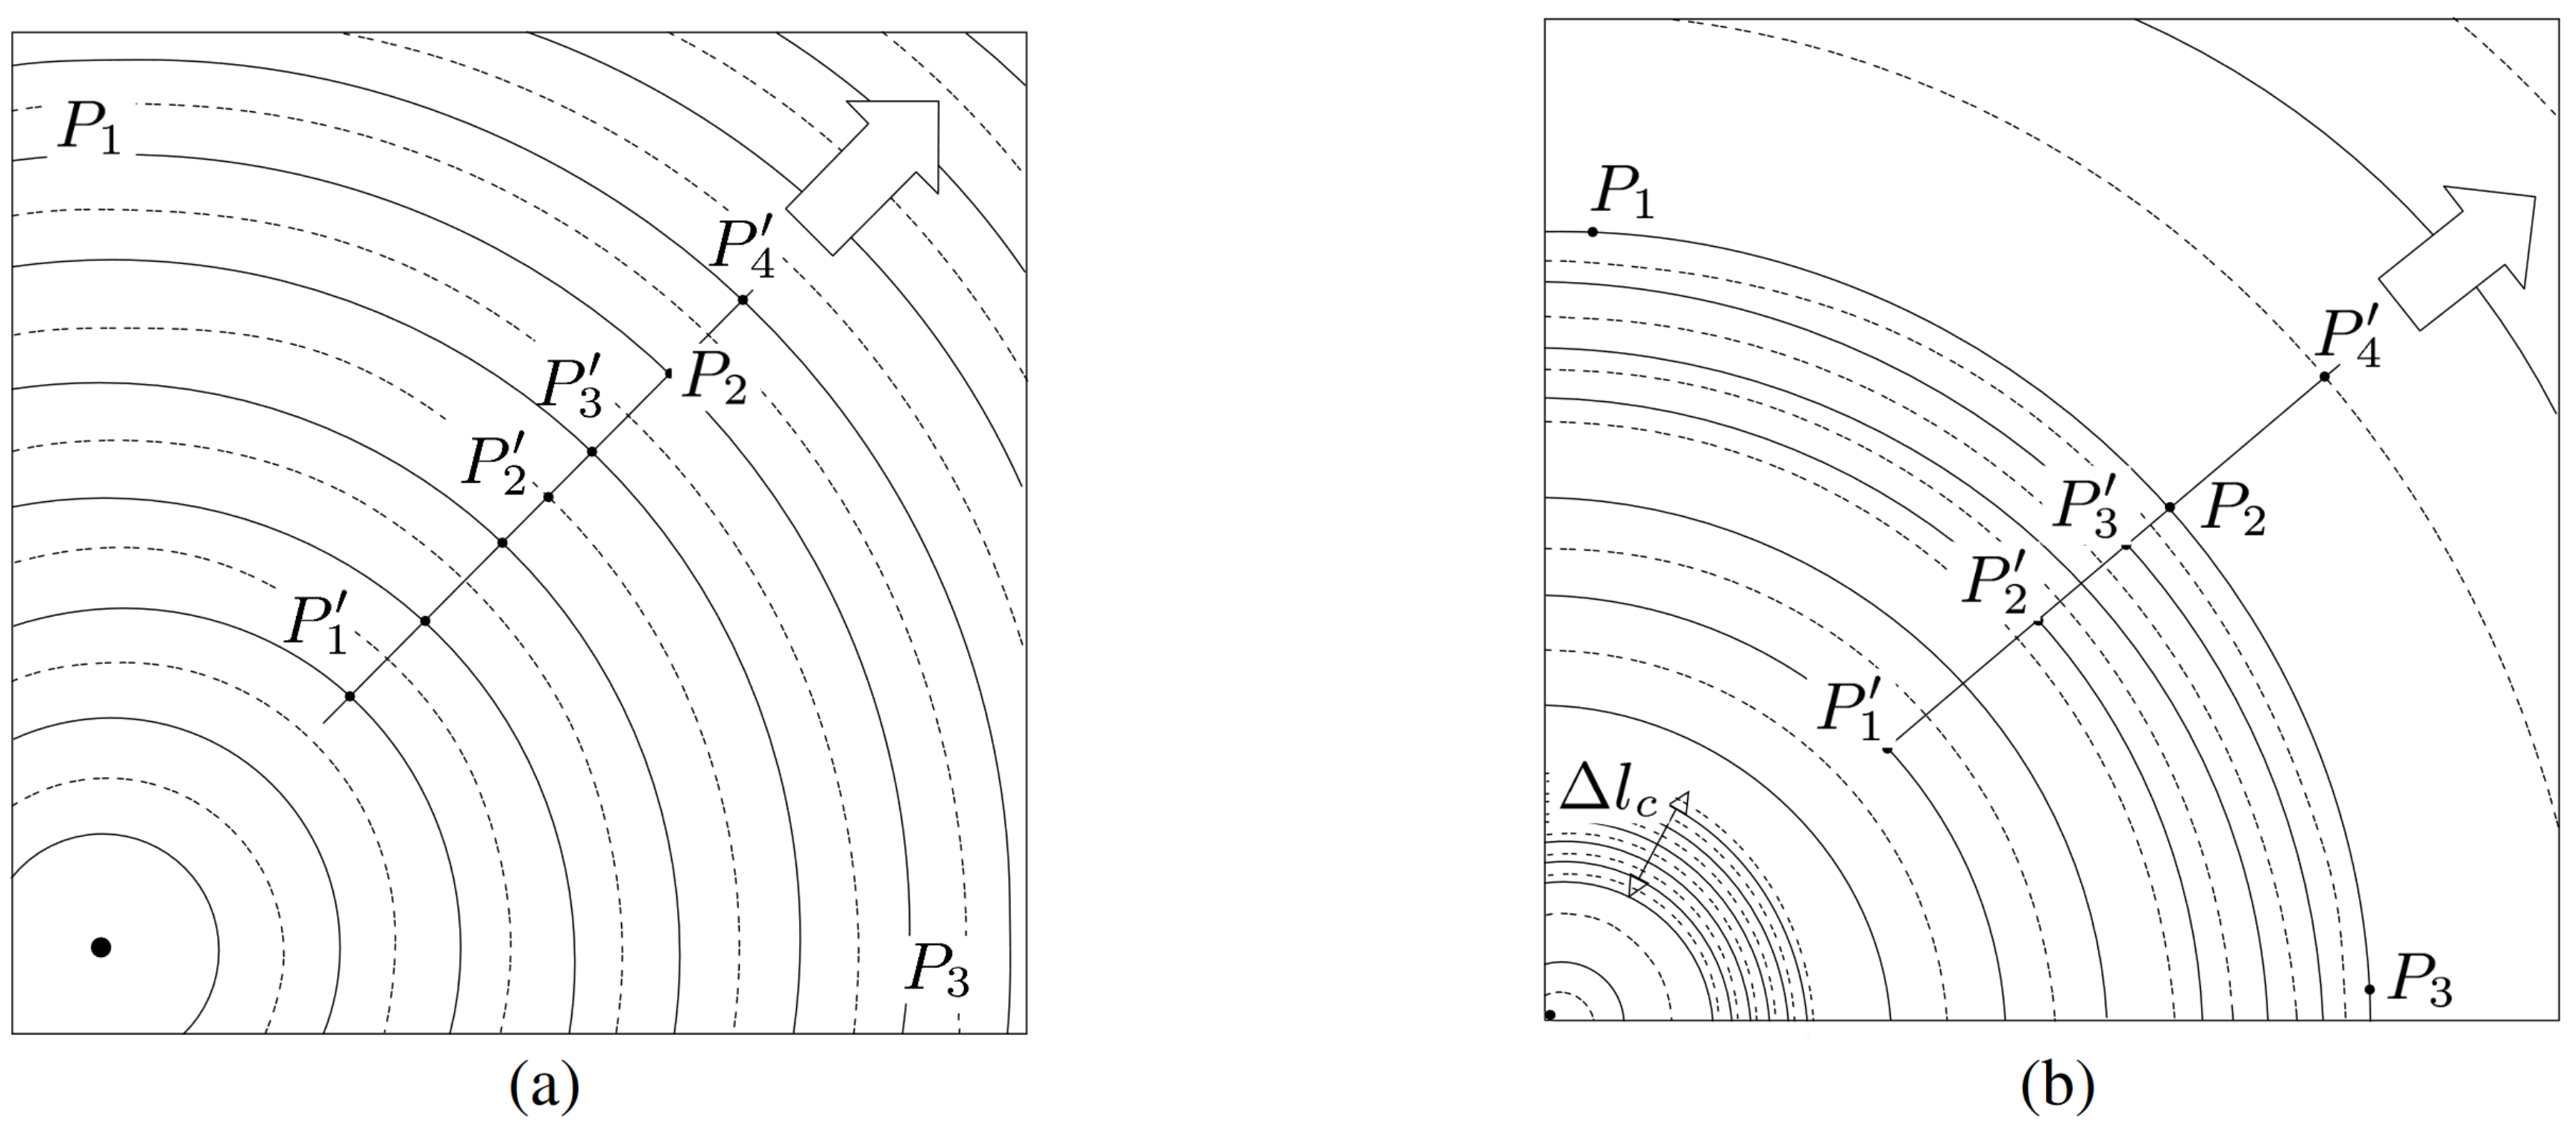
\includegraphics[width=0.8\textwidth]{images/Theorie/Hecht_9.6.png}
    \caption{Dargestellt ist eine Skizze von Wellenfronten zur Veranschaulichung von Kohärenz. In (a) ist die Welle vollständig räumlich und zeitlich kohärent. In (b) ist die Welle nur noch teilweise zeitlich kohärent, aber weiterhin räumlich kohärent. Die Kohärenzlänge $\Delta l_\mathrm{c}$ ist eingezeichnet. Abbildung entnommen aus \cite{hechtOptik2018}.}
    \label{fig:skizze kohärenz}
\end{figure}
\autoref{fig:skizze kohärenz} (a) zeigt eine vollständig kohärente Welle, in welcher Phasenbeziehungen zwischen Punkten in der Ausbreitungsrichtung vollkommen deterministisch sind. 
Die Welle ist monochromatisch und damit zeitlich oder auch longitudinal kohärent. 
Auch in transversaler Richtung (vergleiche Punkte $P_1$-$P_3$) entlang einer Wellenfront ist die Phasenbeziehung für jeden Zeitpukt identisch. 
Die Welle ist räumlich bzw. transversal kohärent. 
Räumliche Kohärenz liegt auch in \autoref{fig:skizze kohärenz} (b) vor. 
Allerdings ist erkennbar, dass die Welle in longitudinaler Richutung nicht für alle Distanzen eine feste Phasenbeziehung aufweist. 
So ist die Frequenz in $P_1'$ beispielsweise niedriger als die in $P_3'$. 
Es existieren aber trotzdem Bereiche, in welchen die Phase sich deterministisch verändert. 
Die kürzeste Länge, für die dies gilt, ist die Kohärenzlänge $\Delta l_\mathrm{c}$, die über die Ausbreitungsgeschwindigkeit $c$ mit der sog. Kohärenzzeit $\Delta l_\mathrm{c} = c\tau_{\mathrm{c}}$ zusammenhängt. 
Die Kohärenzzeit ist damit jene Zeit, für welche die Phase einer Welle vorhersehbar ist. 
Damit haben vollständig zeitlich kohärente Quellen eine unendlich lange Kohärenzzeit, teilweise kohärente Quellen eine endliche Kohärenzzeit, und für inkohärente Quellen gilt $\tau_{\mathrm{c}}\approx 0$. 

Die obige Abbildung motiviert bereits, dass die Kohärenzzeit ein Maß für die spektrale Breite des Lichts $\Delta \omega$ darstellt. 
Es gilt \cite{foxQuantumOpticsIntroduction2006}:
\begin{equation}
    \tau_{\mathrm{c}}  \approx \frac{1}{\Delta \omega}
    \label{eq:tau(delta nu)}
\end{equation}
Da Kohärenz eine Korrelation in den Feldamplituden beschreibt, lässt sich diese Eigenschaft des Lichtes mathematisch mit der sog. Korrelationsfunktion erster Ordnung beschreiben. 
Diese lautet \cite{foellmiIntensityInterferometrySecondorder2009}:
\begin{equation}
    g^{(1)}(\mathbf{r_1}, t_1, \mathbf{r_2}, t_2) = \frac{\left<E^*(\mathbf{r_1}, t_1)E(\mathbf{r_2}, t_2)\right>}{\left[\left<E^*(\mathbf{r_1}, t_1)^2\right> \left<E(\mathbf{r_2}, t_2)^2\right>\right]^{1/2}}
    \label{eq:g1(r1,t1,r2,t2)}
\end{equation}
Hierbei bezeichnet $E(\mathbf{r_i},t_i)$ die komplexe Feldamplitude am Beobachtungsort $\mathbf{r_i}$ und zur Zeit $t_i$ und $\left<\dots\right>$ den Zeitmittelwert über viele Schwingungsperioden. 

Unter der (für weit entfernte, kleine Quellen gerechtfertigten) Annahme, dass die Zeitmittelwerte der Intensitäten an den beiden Orten $\mathbf{r_1}$ und $\mathbf{r_2}$ identisch sind und dass die Intensität zeitlich konstant ist ($\left<I(t_1)\right>=\left<I(t_2)\right>=:I$) lässt sich die Funktion weiter umschreiben. 
Zudem sind häufig nur Differenzen in der Zeit und im Ort relevant, anstatt absolute Orte und Zeiten zu betrachten, was folgende Variablensubstitution nahelegt: $\tau = t_2 -t_1$ und $\bm{\rho} = \mathbf{r_2} - \mathbf{r_1}$. 
Damit folgt:
\begin{equation}
    g^{(1)}(\mathbf{r}, \bm{\rho}, t, \tau) = \frac{\left<E^*(\mathbf{r}, t)E(\mathbf{r}+\bm{\rho}, t+\tau)\right>}{I}
    \label{eq:g1(r1,r2,tau)}
\end{equation}
Häufig wird zudem nur die Korrelation zweier Punkte am selben Ort, d. h. $\bm{\rho}=0$ oder zur selben Zeit, d. h. $\tau=0$, betrachtet. 
Ist dies der Fall, vereinfacht sich \autoref{eq:g1(r1,r2,tau)} zur zeitlichen bzw. räumlichen Korrelationsfunktionen $g^{(1)}(\tau)$ bzw. $g^{(1)}(\bm{\rho})$.


\subsection{Michelson-Sterninterferometer}
\label{ssec:Michelson-Sterninterferometer}
Eine Methode, die räumliche Korrelationsfunktion erster Ordnung zu messen, ist das Michelson-Sterninterferometer, welches schematisch in \autoref{fig:Michelson-Sterninterferometer} dargestellt ist. 
\begin{figure}[h]
    \centering
    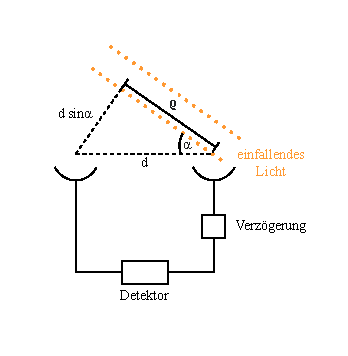
\includegraphics[width=0.65\textwidth]{images/Theorie/Michelson_Interferometer.pdf}
    \caption{Abgebildet ist eine Skizze des Michelson-Sterninterferometers zur Bestimmung von Sternendurchmessern. Zwei durch die Distanz $d$ getrennte Spiegel lenken das Sternenlicht zusammen und es kommt zur Interferenz, die mit einem Detektor beobachtbar ist. Dafür wird der geometrische Streckenunterschied $d\sin\alpha$ durch Verzögerungen kompensiert, um dieselbe Wellenfront zu vergleichen. Abbildung inspiriert von \cite[Abb. 1]{foellmiIntensityInterferometrySecondorder2009}.}
    \label{fig:Michelson-Sterninterferometer}
\end{figure}
Der historische Grund für die Entwicklung von Interferometern zur Beobachtung von Sternen liegt im Ziel, immer bessere Winkelauflösungen erreichen zu wollen. 
Während für die Winkelauflösung gewöhnlicher Teleskope $\theta \propto \frac{\lambda}{D}$ gilt, gilt für Interferometer $\theta \propto \frac{\lambda}{d}$. 
\todo{citation}
Hierbei ist $\lambda$ die Wellenlänge, $D$ der Durchmesser der Teleskopöffnung (je nach Bauart der Hauptspiegel oder die Linse) und $d$ der Abstand zwischen Teleskopen, die ein Interferometer bilden. 
Da es technisch schwierig ist, beliebig große Spiegel- bzw. Linsendurchmesser anzufertigen, sind optische Teleskope auf eine vergleichsweise geringe Auflösung im Bereich von einigen Bogensekunden limitiert. 
Bogensekunden und Bogenminuten (arcsec bzw. arcmin) sind eine typische astronomische Einheit für scheinbare Durchmesser von Objekten in einer gegebenen Entfernung. 
Eine Bogensekunde entspricht dabei dem Sechzigsten Teil einer Bogenminute und eine Bogenminute dem Sechzigsten Teil eines Grades. 
So erreicht z. B. das \emph{Gran Telescopio Canarias} (GTC) eine Auflösung von etwa 12\,marcsec bei $\lambda=500\,\mathrm{nm}$ und $D=10{,}4\,\mathrm{m}$ \cite{GranTelescopioCANARIAS}. 
Obwohl es Bestrebungen gibt, immer größere Einzelspiegelteleskope zu bauen, besteht eine weitere, technisch einfachere Herangehensweise darin, das Licht vieler kleiner Teleskope zu kombinieren. 
Dies ist die Grundidee des Michelson-Sterninterferometers, welches aus zwei Teleskopen besteht, die durch eine Distanz $d$ voneinander getrennt sind. 
Diese bündeln das Licht, welches anschließend zusammengeführt und zur Interferenz gebracht wird. 
Durch dieses Vorgehen lassen sich deutlich bessere Winkelauflösungen bewerkstelligen. 
So erreichte z. B. das Ende der 1980er gebaute \emph{Sydney University Stellar Interferometer} (SUSI) Auflösungen von $70\,\mathrm{\mu arcsec}$ bei $\lambda=450\,\mathrm{nm}$ und $d=640\,\mathrm{m}$ \cite{davisSydneyUniversityStellar1999}. 
Ein Nachteil des Interferometers ist allerdings eine niedrigere Sensitivität im Vergleich zu gewöhlichen Teleskopen. 
Da die Lichtsammelfläche zweier kleiner Teleskope für gewöhnlich kleiner ist als die eines großen Einzelspiegels, wird weniger Licht gesammelt, was interferometrische Verfahren auf vergleichsweise helle Sterne limitiert \cite[Kap. 6.1]{foxQuantumOpticsIntroduction2006}. 
Weiterhin wird statt eines zweidimensionalen Bildes lediglich eine eindimensionale Größe, nämlich der Winkeldurchmesser des Sternes, bestimmt. 
Durch den Zusammenschluss vieler Teleskope kann allerdings trotzdem auf die zweidimensionale Helligkeitsverteilung rückgeschlossen werden. 
Weiterführendes findet man unter dem Stichpunkt \glqq Aperture Synthesis\grqq\;z. B. in \cite[Kap. 10]{burkeIntroductionRadioAstronomy2019}. \\

Beobachtungsziel des Interferometers ist ein Stern, also eine ausgedehnte, thermische Lichtquelle. 
Thermisches Licht ist zwar grundsätzlich nicht kohärent, aber ein Gedankenexperiment zeigt auf, dass durch das Samplen des Lichts an zwei weit vom Stern entfernten Orten trotzdem teilweise Kohärenz vorliegen kann. 
Man kann sich eine ausgedehnte Lichtquelle als die Superposition vieler infinitesimal kleiner Quellen vorstellen. 
Jede dieser Punktquellen hat für sich genommen keine Winkelausdehnung und bildet damit im Fernfeld eine vollständig räumlich kohärente ebene Welle \cite[Kap. 6.1]{foxQuantumOpticsIntroduction2006}. 
Die Überlagerung der Punktquellen bedeutet nun im Fernfeld eine Überlagerung vieler für sich genommen räumlich kohärenten, aber untereinander inkohärenten ebenen Wellen. 
Da in jedem Teleskop des Interferometers eine Vielzahl dieser ebenen Wellen detektiert wird, verbleibt eine gewisse Ähnlichkeit zwischen den detektierten Feldern -- die beiden Felder sind teilweise korreliert. 
Dies ist in \autoref{fig:räumliche kohärenz einer ausgedehnten quelle} dargestellt. 
\begin{figure}[h]
    \centering
    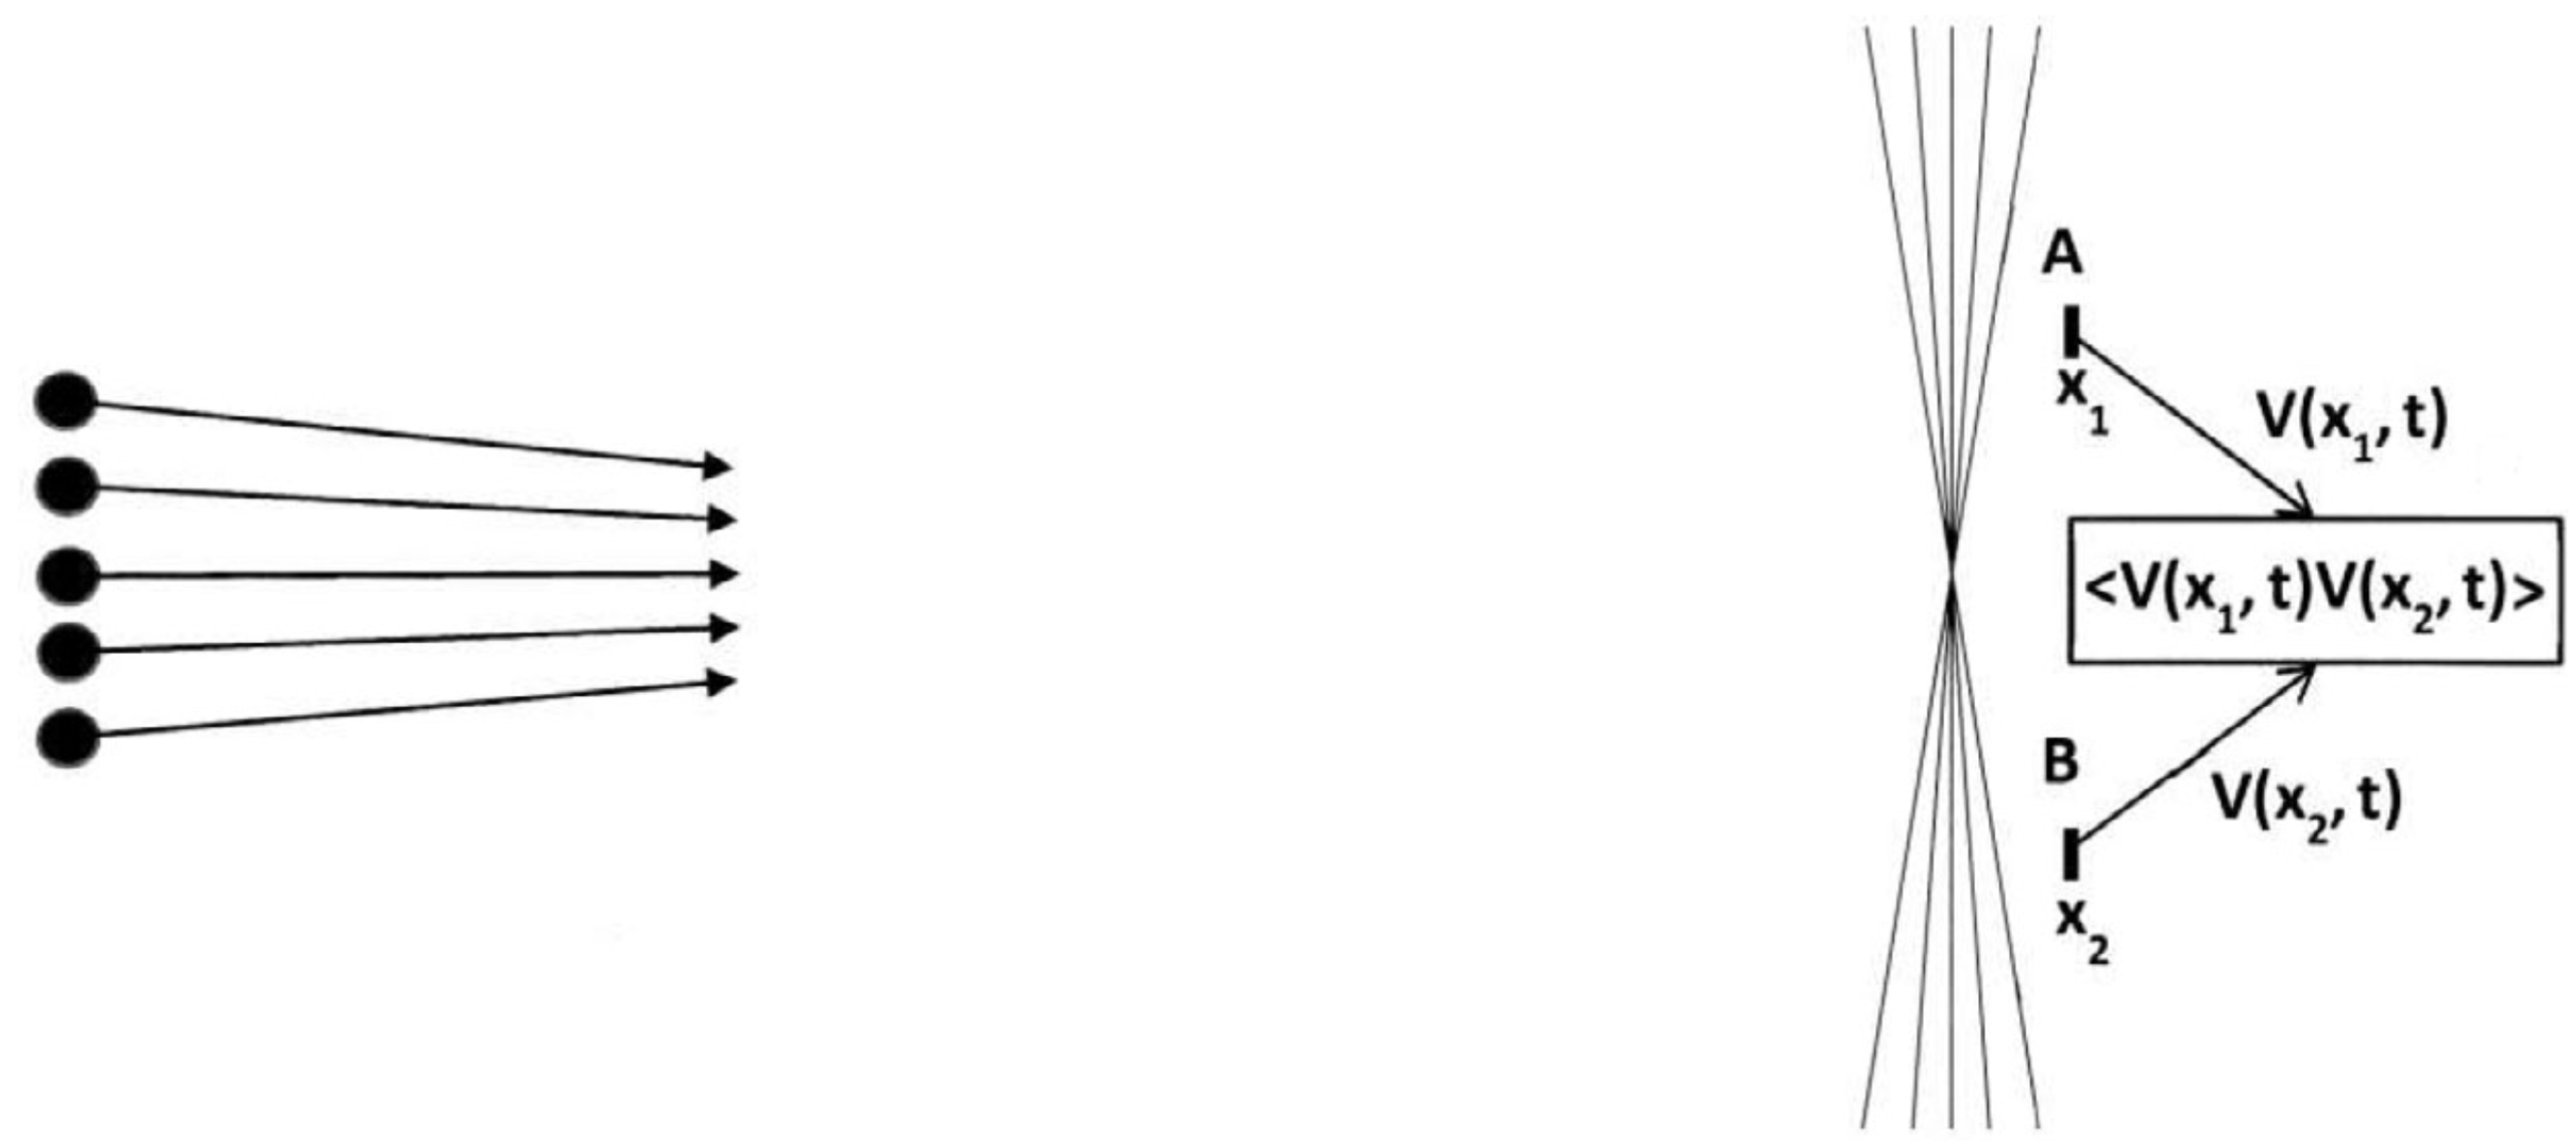
\includegraphics[width=0.8\textwidth]{images/Theorie/Burke_9.25.png}
    \caption{Abgebildet ist eine Skizze, die veranschaulicht, wie eine ausgedehnte inkohärente Quelle bei Teleskopseparationen $d>0$ trotzdem teilweise korreliertes Licht aufweist. Links ist eine Quelle schematisch in viele kohärente Punktquellen zerlegt, die ebene Wellen emittieren. In den beiden Detektoren rechts werden jeweils alle ebenen Wellen detektiert, allerdings kommen diese aufgrund der Geometrie zu leicht verschiedenen Zeiten an. Es ist deutlich, dass die Lichtfelder für steigende $d$ immer verschiedener werden (die Kohärenz sinkt), während sie für $d=0$ vollkommen identisch und somit kohärent sind. Die Abbildung ist \cite[Fig. 9.25]{burkeIntroductionRadioAstronomy2019} entnommen.}
    \label{fig:räumliche kohärenz einer ausgedehnten quelle}
\end{figure}
Diese Korrelation ist maximal für eine Teleskopseparation von $d=0$, da in diesem Fall in beiden Teleskopen exakt dasselbe Licht gemessen wird. 
Wird $d$ nun immer weiter erhöht, verringert sich die Korrelation zwischen den Feldern immer weiter. 
Die Lichtfelder bestehen aus immer verschiedeneren ebenen Wellen und sind sich weniger ähnlich. 
Ab einer Separation $d_0 \approx \Delta l_\mathrm{c}$ sind die Lichtfelder nicht mehr korreliert und $g^{(1)}$ fällt auf Null ab. 
Distanzen entlang der Ausbreitungsrichtung ($l_\mathrm{c}$) und transversal dazu $d_0$ werden im Michelson-Interferomter verknüpft, da die Lichtwellen von verschiedenen Orte zu einem Ort zusammengeführt werden müssen.
Dies schafft eine enge Verbindung zwischen transversaler (räumlicher) und longitudinaler (zeitlicher) Kohärenz.  
Für spektral breites Licht (wie für thermisches Licht von Sternen üblich) ist die Kohärenzlänge und damit die maximale Teleskopseparation sehr klein (vgl. \autoref{eq:tau(delta nu)}). 
Daher wird häufig auf entsprechend enge optische Filter zurückgegriffen, die die spektrale Breite des Lichts heruntersetzen, um die Kohärenzlänge zu erhöhen. \\


Messgröße des Michelson-Sterninterferometers ist im einfachsten Fall der Interferenzkontrast, definiert als \cite{foellmiIntensityInterferometrySecondorder2009}
\begin{equation}
    K = \frac{I_{\mathrm{max}}-I_{\mathrm{min}}}{I_{\mathrm{max}}+I_{\mathrm{min}}}=\left|g^{(1)}(\mathbf{r}, \bm{\rho}, t, \tau)\right|
\end{equation} 
Hierbei sind $I_{\mathrm{max}}$ bzw. $I_{\mathrm{min}}$ die Intensitätsmaxima bzw. -minima der gemessenen Intensität auf dem Schirm. 
$\tau$ ist hierbei die Zeitdifferenz zwischen den beiden Feldern, die durch die Strecke $d\cdot\sin \alpha$ in \autoref{fig:Michelson-Sterninterferometer} entsteht, und $\bm{\rho}$ der effektive Abstandsvektor zwischen den Teleskopen. 
Der effektive Teleskopabstand entspricht der Projektion des Teleskopabstandes $d$ in die Beobachtungsebene, die i. A. nicht parallel zu $d$ liegt. 
Durch komplexere Methoden lässt sich neben der Amplitude auch die Phase der komplexen Funktion $g^{(1)}(\mathbf{r}, \bm{\rho}, t, \tau)$ messen, vgl. dazu \cite[Kap. 4.3]{mandelOpticalCoherenceQuantum1995}. \\
Die Messung eines Sternendurchmessers lässt sich nun wie folgt bewerkstelligen:
Im Interferometer wird die Weglängendifferenz $d \cdot\sin \alpha$ durch die Wahl einer passenden Verzögerung kompensiert, sodass die Welle zwar an zwei verschiedenen Orten, aber effektiv zu ein und derselben Zeit gesampelt wird. 
$\tau=0$ und die Welle ist zeitlich kohärent \cite{foellmiIntensityInterferometrySecondorder2009}. 
Durch Messung des Interferenzkontrastes für verschiedene effektive Spiegelseparationen $\rho=|\bm{\rho}|$ lässt sich die räumliche Korrelationsfunktion erster Ordnung messen. 
Über das van Cittert-Zernike-Theorem lässt sich aus der gemessenen räumlichen Korrelationsfunktion nun über eine Fouriertransformation auf die Intensitätsverteilung der Quelle zurückschließen \cite[Gl. 4.4-40]{mandelOpticalCoherenceQuantum1995}:
\begin{equation}
    g^{(1)}(\bm{r}_1, \bm{r}_2) = \frac{\int_\sigma I(\bm{r}') \,\mathrm{e}^{-i\overline{k}\left(\bm{s}_2 - \bm{s}_1\right) \bm{r}'} d^2r'}{\int_\sigma I \left(\bm{r}'\right) d^2 r'}
    \label{eq:van Cittert-Zernike}
\end{equation}
Hierbei sind $\bm{r}_1=\bm{s}_1 r_1$ und $\bm{r}_2=\bm{s}_2 r_2$ die Verbindungsvektoren zwischen den Beobachtungsorten und einem Punkt der Quelle. 
Es erfolgt eine Integration der Intensität über alle Punkte der Quelle, d. h. alle $I\left(\bm{r}'\right)$ für alle $\bm{r}'\in \sigma$. 
$\overline{k}$ ist die durchschnittliche Wellenzahl des beobachteten Lichts an beiden Orten, d. h. $\overline{k} = \frac{2\pi\overline{\nu}}{c}$ mit der durchschnittlichen Frequenz $\overline{\nu}$ und der Ausbreitungsgeschwindigkeit $c$. 
Die erwähnten Größen sind zur Veranschaulichung ebenfalls in \autoref{fig:van Cittert-Zernike} skizziert. 
\begin{figure}[h]
    \centering
    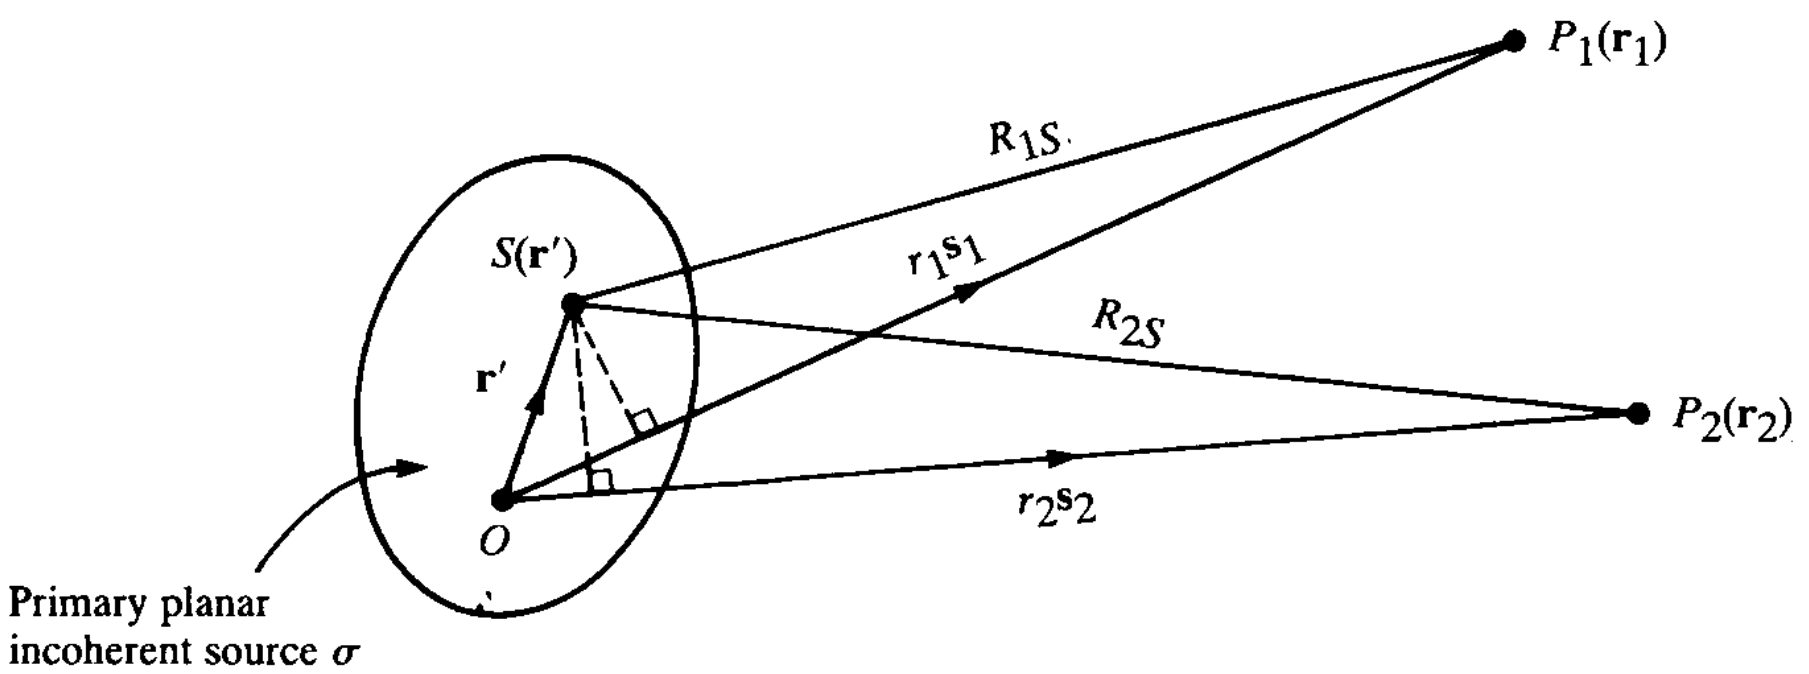
\includegraphics[width=0.8\textwidth]{images/Theorie/Mandel_4.12.png}
    \caption{Veranschaulichung der Größen aus \autoref{eq:van Cittert-Zernike}, entnommen aus \cite[Abb. 4.12]{mandelOpticalCoherenceQuantum1995}. Links ist die Quelle $\sigma$ zu sehen, während die Punkte $P_1$ und $P_2$ die Beobachtungsorte darstellen sollen. }
    \label{fig:van Cittert-Zernike}
\end{figure}
Der Vollständigkeit halber soll hier auch auf die Rolle der zeitlichen Korrelation $g^{(1)}(\tau)$ eingegangen werden. 
Diese stellt zwar bei interferometrischen Beobachtungen selten die primäre Observable dar, enthält aber trotzdem Informationen über die Quelle. 
Während die räumliche Korrelationsfunktion erster Ordnung mit dem Intensitätsprofil der Quelle zusammenhängt, gilt für $g^{(1)}(\tau)$ das Wiener-Khintchine-Theorem \cite{lasseguesFieldIntensityCorrelations2022}:
\begin{equation}
    S(\omega) =  \int g^{(1)}(\tau) e^{i\omega\tau} d\tau
\end{equation}
Das Spektrum der Quelle $S(\omega)$ ist die Fouriertransformierte der zeitlichen Korrelationsfunktion erster Ordnung. \\
Auch wenn wie erwähnt $g^{(1)}(\tau)$ häufig nicht die primäre Observable ist, soll hier noch einmal explizit erwähnt werden, dass für eine interferometrische Beobachtung nie \emph{nur} die räumliche Kohärenz der Quelle ausschlaggebend ist. 
Um nicht verschwindende räumliche Kohärenz messen zu können, muss $d\lesssim \Delta l_\mathrm{c}$ gelten, d. h. eine gewisse zeitliche Kohärenz vorherrschen. 
Nach \autoref{eq:tau(delta nu)} ist dies zu erreichen indem das Licht durch optische Filter spektral so verengt wird, dass ausreichend zeitliche Kohärenz vorliegt. 
Es ist ersichtlich, dass räumliche und zeitliche Kohärenz eng verknüpfte Konzepte darstellen, die lediglich in der Theorie klar getrennt sind. 
Daher ist es nicht verwunderlich, dass die Notwendigkeit spektraler Filter zur Herstellung zeitlicher Kohärenz auch bei der Einführung der Intensitätsinterferometrie in \autoref{ssec:Intensitätsinterferometrie} von Belang sein wird, obwohl die Begriffe Kohärenzzeit und -länge weniger klar deutbar sind. \\

Ein Nachteil des Michelson-Sterninterferometers ist die schwierig herzustellende Stabilität im Teleskop. 
Da die Wellen direkt miteinander interferieren, muss der Weg des Lichts auf einen Bruchteil einer Wellenlänge stabilisiert werden, um Phasenstabilität sicherzustellen. 
Dies wird insbesondere schwieriger, je größer die Spiegelabstände werden, was das Herstellen großer Winkelauflösungen erschwert. 
Weiterhin induzieren atmosphärische Variabilitäten schwer vorherzusagende Phasendifferenzen zwischen den beiden Teleskopen, die das Interferenzenmuster beeinflussen \cite[Kap. 2]{brownIntensityInterferometerIts1974}. 
Durch dieses sogenannte \glqq Seeing\grqq\;und die Notwendigkeit eines mechanisch sehr präzisen und stabilen Aufbaus sind Michelson-Sterninterferometer in ihrer Größe limitiert. 
Um beide Probleme zu umgehen, haben Hanbury Brown und Twiss ein modifiziertes System entwickelt -- das Intensitätsinterferometer.

\subsection{Intensitätsinterferometrie}
\label{ssec:Intensitätsinterferometrie}
Im Gegensatz zum Michelson-Sterninterferometer, in dem die Amplituden der Lichtwellen direkt zur Interferenz gebracht werden, werden im von Hanbury Brown und Twiss erstmals 1955 im Labor durchgeführten Experiment \cite{brownCorrelationPhotonsTwo1956} die Intensitäten direkt mit zwei Photomultipliern gemessen. 
Anschließend werden anstatt der Lichtwellen direkt die Photoströme miteinander korreliert. 
Bereits in den 1960ern und 70ern entwickelten Hanbury Brown und Twiss auf das erfolgreiche Laborexperiment und weitere Tests folgend das erste Intensitätsinterferometer, das \emph{Narrabi Stellar Intensity Interferometer} und bestimmten die Winkeldurchmesser von 32 Sternen \cite[Kap. 1]{brownIntensityInterferometerIts1974}. \\
Dies war nur möglich aufgrund des vergleichsweise einfachen Aufbaus. 
An beiden Teleskopen wird voneinander unabhängig der Photonenstrom, z. B. mittels Photomultipliern, gemessen und anschließend elektronisch korreliert. 
Vor- und Nachteil dieser Vorgehensweise ist die Insensitivität gegenüber Phasenunterschieden zwischen dem eintreffenden Licht an beiden Teleskopen. 
Einerseits geht durch die Messung Information (über die Phase) verloren, andererseits wird der Aufbau einfacher, da weder Phasenstabilität zwischen Teleskopen noch atmosphärisches Seeing einen Einfluss auf das korrelierte Signal haben.
Dieses Vorgehen ermöglicht im Prinzip beliebig lange Separationen und damit beliebig gute Winkelauflösungen. 
Vorraussetzung dafür ist lediglich, die Distanz zwischen Teleskopen im Vergleich zur Länge, die das Licht in der Detektorzeitauflösung zurücklegt, genau zu kennen \cite{DemonstrationStellarIntensity}. 
%So werden mit den VERITAS-Teleskopen z. B. mittels Intensitätsinterferometrie von Licht mit der Wellenlänge $\lambda_{\mathrm{eff}}=416\,\mathrm{nm}$ und effektiven, maximalen Teleskopseparationen von $r_{\mathrm{avg}}=157{,}9\,\mathrm{m}$ Winkelauflösungen von etwa $0{,}6\,\mathrm{marcsec}$ erreicht \cite{DemonstrationStellarIntensity}.
\\
Eine schematische Darstellung des Intensitätsinterferometers ist in \autoref{fig:Intensitätsinterferometer} dargestellt. 
\begin{figure}[h]
    \centering
    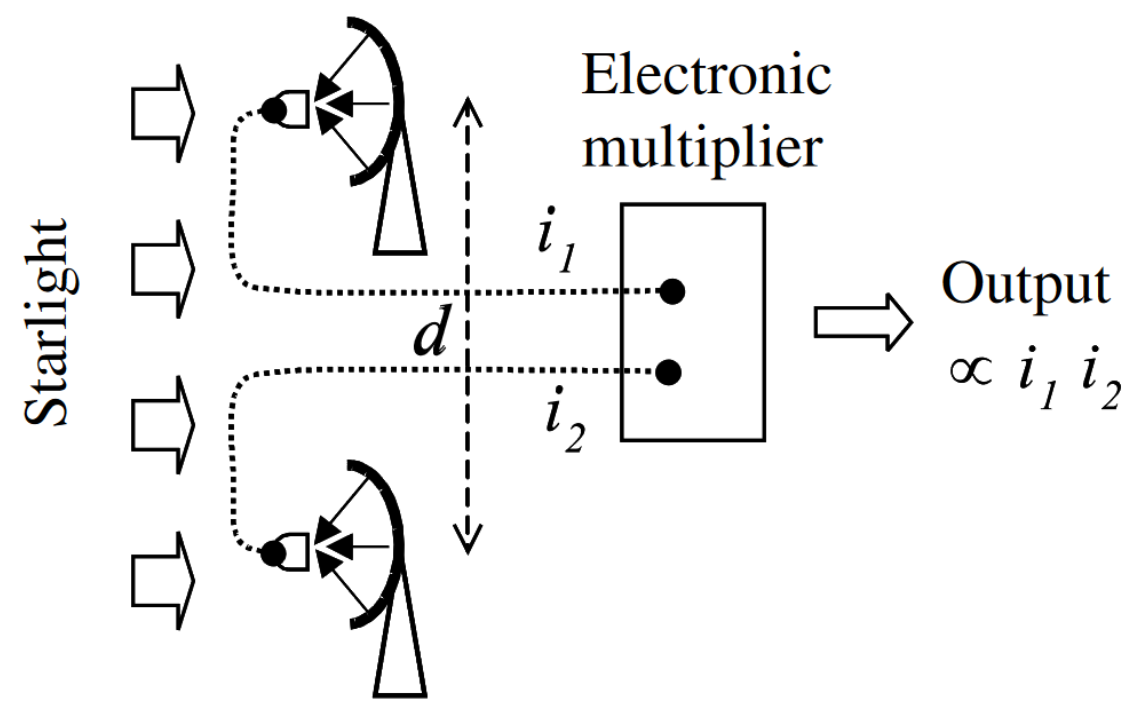
\includegraphics[width=0.65\textwidth]{images/Theorie/Fox_6.1b.png}
    \caption{Eine Skizze des Intensitätsinterferometers ist abgebildet. Das gesammelte Licht wird direkt detektiert und das zu den Intensitäten proportionale Signal elektronisch kombiniert. Entnommen aus \cite[Fig. 6.1(b)]{foxQuantumOpticsIntroduction2006}.}
    \label{fig:Intensitätsinterferometer}
\end{figure}
Zur Beschreibung der Korrelation von Intensitäten ist eine Erweiterung der bisher genannten Theorie nötig. 
Es bietet sich an, eine Korrelationsfunktion zweiter Ordnung einzuführen. 
Diese lässt sich erneut in relativen Abständen definieren, sodass $\bm{\rho} = \mathbf{r_2} - \mathbf{r_1}$ und $\tau = t_2 - t_1$, womit folgt (vgl. \cite{foellmiIntensityInterferometrySecondorder2009}):
\begin{equation}
    g^{(2)}(\mathbf{r}, t, \bm{\rho}, \tau) = \frac{\left<E^*(\mathbf{r}, t)E^*(\mathbf{r}+\bm{\rho}, t+\tau)E(\mathbf{r}+\bm{\rho}, t+\tau)E(\mathbf{r}, t)\right>}
        {\left<E^*(\mathbf{r}, t)E(\mathbf{r}, t)\right>^2}
\end{equation}
Mit der Notation $I=\left<I(t)\right>$ und unter der Annahme von thermischem, bzw. chaotischem Licht, in dem die Phasen der emittierten Lichtquanten zufällig verteilt sind, folgt:
\begin{equation}
    g^{(2)}(\mathbf{r}, \bm{\rho}, t, \tau) =  \frac{\left<I(\mathbf{r}, t) I(\mathbf{r}+\bm{\rho}, t+\tau)\right>}{I^2}
    \label{eq:g2_final}
\end{equation}
Durch das Interferometer kann nun (analog zu $g^{(1)}(\bm{\rho})$ beim Michelson-Sterninterferometer) $g^{(2)}(\bm{\rho})$ gemessen werden. 
Um nun trotzdem auf die Quellengeometrie schließen zu können, wird ein Zusammenhang zwischen $g^{(1)}$ und $g^{(2)}$, die sog. Siegert-Relation, genutzt \cite{lasseguesFieldIntensityCorrelations2022}:
\begin{equation}
    g^{(2)}(\tau) = 1+ \left|g^{(1)}(\tau)\right|^2
\end{equation}
Diese gilt nur für chaotisches und thermisches Licht. 
Unter chaotischem Licht versteht man Licht, dessen Quanten aufgrund von Stößen unter emittierenden Gasmolekülen und der Eigenbewegung dieser mit zufälliger Phase emittiert werden. 
Es weist ähnlich wie thermisches Licht, welches Schwarzkörperstrahlung entspricht, Intensitätsschwankungen auf der Zeitskala einer Kohärenzzeit auf. 
Ein Beispiel für thermisches Licht ist die Emission eines Sterns und ein Beispiel für chaotisches Licht das Licht einer Gasentladungslampe \cite{foxQuantumOpticsIntroduction2006}. \\
Über eine Messung von $g^{(2)}$ mit dem Intensitätsinterferometer kann also mit der Siegert-Relation auf $\left|g^{(1)}\right|$ geschlossen werden. 
Da die Phaseninformation von $g^{(1)}$ durch dieses Vorgehen unbekannt ist, kann nicht direkt durch Anwendung des van Cittert-Zernike-Theorems auf die Quellengeometrie geschlossen werden. 
Stattdessen wird üblicherweise ein Modell der Lichtquelle angenommen, von welchem die Fouriertransformation bekannt ist. 
Durch einen Fit dieser an die gemessenen Daten lassen sich abschließend physikalische Größen wie der Durchmesser der Quelle bestimmen. \\
Ein Beispiel für typische im Labor auftretende Größenordnungen der räumlichen Korrelationsfunktionen ist in \autoref{fig:g1(rho),g2(rho) für versch Lochblenden} dargestellt. 
Hierbei wird als \glqq Stern\grqq\;eine von einer chaotischen Lichtquelle uniform ausgeleuchtete Lochblende des Durchmessers $d$ im Abstand $x$ angenommen. 
Dies entspräche im einfachsten Sternmodell einer uniform leuchtenden Scheibe einem Stern mit Winkeldurchmesser $\Delta \theta = \frac{d}{x}$. 
Für dieses Modell gilt nach \cite[Kap. 4.1]{brownIntensityInterferometerIts1974}:
\begin{align}
    \left| g^{(1)}(\rho)\right| &= \frac{2J_1\left(\frac{\pi\rho\Delta\theta}{\lambda_0}\right)}{\frac{\pi\rho\Delta\theta}{\lambda_0}}\quad\quad\quad \Rightarrow & g^{(2)}(\rho) &= 1 + \left[\frac{2J_1\left(\frac{\pi\rho\Delta\theta}{\lambda_0}\right)}{\frac{\pi\rho\Delta\theta}{\lambda_0}}\right]^2
\end{align}
Hierbei sind $J_1$ die Besselfunktion erster Ordnung und $\lambda_0$ die zentrale Wellenlänge, gegeben durch den verwendeten Filter. 
Für Werte von $x=1{,}75\,\mathrm{m}$ und $\lambda_0=465\,\mathrm{nm}$ ergeben sich die in \autoref{fig:g1(rho),g2(rho) für versch Lochblenden} gezeigten Verläufe. 
\begin{figure}[h]
    \centering
    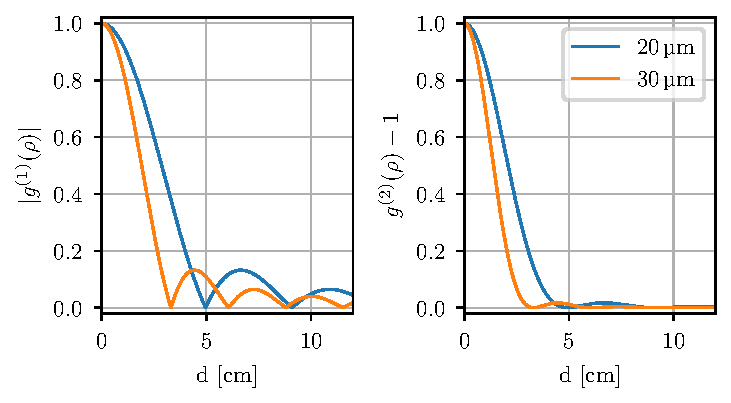
\includegraphics{images/Theorie/g1_g2_rho.pdf}
    \caption{Gezeigt sind die Verläufe von $g^{(1)}(\rho)$ und $g^{(2)}(\rho)$ für zwei Lochblenden mit Durchmesser $20\,\mathrm{\mu m}$ und $30\,\mathrm{\mu m}$. Für beide Lochblenden ist $x=1{,}75\,\mathrm{m}$ und $\lambda_0=465\,\mathrm{nm}$.}
    \label{fig:g1(rho),g2(rho) für versch Lochblenden}
\end{figure}
Durch Samplen der Funktion $g^{(2)}(\rho)$ kann die erste Nullstelle bestimmt werden, die für das genannte Modell bei 
\begin{equation}
    \rho_0=1{,}22\frac{\lambda_0}{\Delta\theta} 
    \label{eq:erste nulstelle von g2(rho) für lochblende}
\end{equation}
liegt \cite[Kap. 4.1]{brownIntensityInterferometerIts1974}. 
Aus dieser kann dann der Winkeldurchmesser berechnet werden. 
Es ist ersichtlich, dass typische Größenordungen von $\rho_0$ im Labor bei wenigen Zentimetern liegen, während bei Sternen Separationen im Bereich von hundert Metern bis zur ersten Nullstelle üblich sind (vgl. z. B. \cite[Abb. 10.2]{brownIntensityInterferometerIts1974}). \\


Um $g^{(2)}(\rho)$ für verschiedene effektive Teleskopseparationen zu samplen, wird für jede Distanz $\rho=|\bm{\rho}|$ die zeitliche Korrelationsfunktion zweiter Ordnung gemessen, indem die gemessenen Intensitäten miteinander korreliert werden. 
Deswegen soll im Folgenden der erwartete Verlauf der Observablen $g^{(2)}(\tau)$ näher beschrieben werden. 
Anhand des Verhaltens von $g^{(2)}(0)$ lassen sich drei Phänomene unterscheiden \cite{foxQuantumOpticsIntroduction2006}. 
\begin{itemize}
    \item $g^{(2)}(0)=1$: Die Photonen treffen mit zufälligen Abständen auf den Detektor. Das Licht ist kohärent und es gilt allgemein $g^{(2)}(\tau)=1$. Dies gilt für einen idealen, monochromatischen Laser \cite[Kap. 9]{mansuripurClassicalOpticsIts2009}.
    \item $g^{(2)}(0)>1$: Die Photonen erreichen die Detektoren gebündelt in sog. \emph{bunches}. Die Korrelation ist erhöht bei niedrigen Zeitdifferenzen. Mit anderen Worten ist es also wahrscheinlicher, ein weiteres Photon zu messen, wenn zuvor bereits eines gemessen wurde. Thermisches und chaotisches Licht zeigen Bunching.
    \item $g^{(2)}(0)<1$: Die Photonen treffen in regelmäßigen Abständen auf den Detektor. Es ist daher unwahrscheinlicher als im kohärenten Fall, kurz nach der Messung eines Photons ein weiteres zu messen. Dieses Phänomen bezeichnet man als Antibunching. 
\end{itemize}
Eine Veranschaulichung der Einteilung des Lichtes ist in \autoref{fig:bunching} gezeigt. 
\begin{figure}[h]
    \centering
    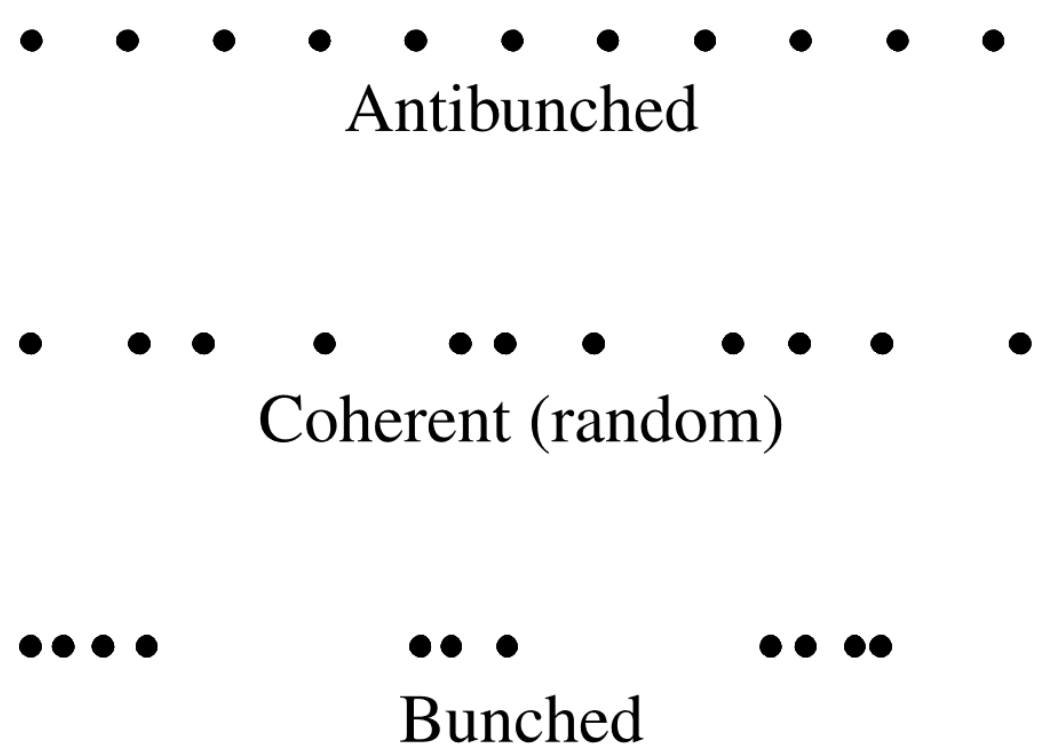
\includegraphics[width=0.4\textwidth]{images/Theorie/Fox_6.6.png}
    \caption{Anitbunching, kohärente Photonen und Bunching sind schematisch dargestellt. Während die Photonenabstände bei kohärentem Licht zufällig sind, sind bei Antibunching regelmäßige und bei Bunching geringe Abstände wahrscheinlicher. Abbildung aus \cite[Abb. 6.6]{foxQuantumOpticsIntroduction2006}}
    \label{fig:bunching}
\end{figure}
Eine weitere geläufige Einteilung des Lichts wird aufgrund der Photonenstatistik, also der Verteilung der gemessenen Einzelphotonen in einem gewissen Zeitintervall, vorgenommen. 
Nach dieser Einteilung ist die Anzahl gemessener kohärenter Photonen poissonverteilt, während gebunchte Photonen einer breiteren und antigebunchte Photonen einer schmaleren Verteilung folgen. 
Eine tiefergehende Beschreibung findet sich z. B. in \cite[Kap. 5.4-5.6]{foxQuantumOpticsIntroduction2006}. \\

Durch die Siegert-Relation und den bereits beschriebenen Verlauf von $g^{(1)}(\tau)$ lässt sich auf das Aussehen von $g^{(2)}(\tau)$ schließen (vgl. \cite[Kap. 6.3]{foxQuantumOpticsIntroduction2006}). 
So ist bei einem idealen Detektor $g^{(2)}(0)=2$ und fällt für $|\tau|>0$ immer weiter ab, bis sich $g^{(2)}$ nach einer Zeit in der Größenordnung der Kohärenzzeit, also für $\tau\gtrsim\tau_{\mathrm{c}}$, dem Wert 1 annähert. 
Da $g^{(2)}(\tau)$ bei chaotischen Lichtquellen wie bereits erwähnt über eine Fouriertransformation mit dem Spektrum der Quelle zusammenhängt, ergibt sich je nach verwendetem Filter ein anderer Verlauf von $g^{(2)}(\tau)$ zwischen dem Wert 2 und 1. 
Ein beispielhafter Verlauf von $g^{(1)}(\tau)$ und $g^{(2)}(\tau)$ ist in \autoref{fig:g1(tau),g2(tau) für versch Filter} für einen Filter mit rechteckigem Transmissionsprofil, zentraler Wellenlänge $\lambda_0 = 465\,\mathrm{nm}$ und Breiten $\Delta\lambda$ von 2\,nm und 5\,nm aufgezeigt. 
Für die normalisierte Fouriertransformation einer Rechteckfunktion $\mathrm{rect}_{\Delta f}\left(f\right)$ und damit $g^{(1)}(\tau)$ gilt (vgl. \cite[Kap. 3.2]{wangIntroductionOrthogonalTransforms2012}):
\begin{align}
    g^{(1)}(\tau) &= \mathrm{sinc}\left(\tau\Delta f\right) \quad\quad\quad \Rightarrow& g^{(2)}(\tau) &= 1+ \left[\mathrm{sinc}\left(\tau\Delta f\right)\right]^2
\end{align}
Hierbei entspricht $\Delta f$ der Umrechnung von $\Delta\lambda$ in den Frequenzraum, d. h. 
\begin{equation}
    \Delta f = \frac{c}{\lambda_0 - \nicefrac{\Delta\lambda}{2}} - \frac{c}{\lambda_0 + \nicefrac{\Delta\lambda}{2}}
\end{equation}
\begin{figure}[h]
    \centering
    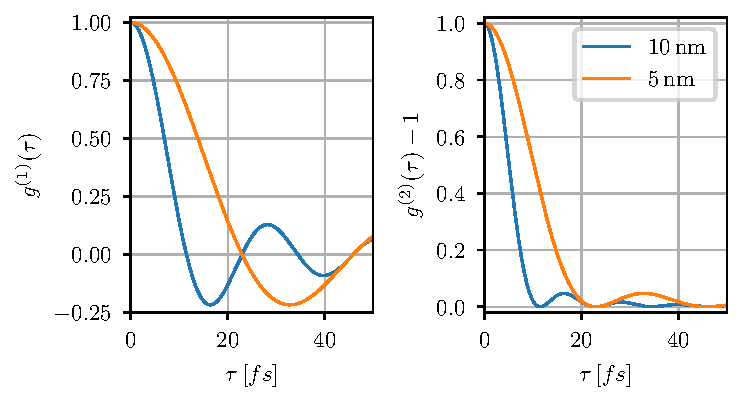
\includegraphics{images/Theorie/g1_g2_tau.pdf}
    \caption{Abgebildet ist der Theorieverlauf von $g^{(1)}(\tau)$ und $g^{(2)}(\tau)$ für einen Filter mit rechteckigem Transmissionsprofil mit Breite 2, bzw. 5\,nm, zentriert um 465\,nm.}
    \label{fig:g1(tau),g2(tau) für versch Filter}
\end{figure}
In einer realen Messung verringert das Binning der Messdaten in Intervalle $\tau_\mathrm{B}$ den Wert von $g^{(2)}(0)$ zusätzlich. 
Da dieses zumeist deutlich größer ist als die Kohärenzzeit, werden im zentralen Bin $\tau \in [0, \tau_\mathrm{B}]$ neben den kohärenten Photonen auch ein Faktor $\nicefrac{\tau_\mathrm{B}}{\tau_{\mathrm{c}}}$ mehr zufällig koinzidente Photonen gemessen. 
Dies verringert $g^{(2)}(0)$ um ebendiesen Faktor \cite[Kap. 14.7]{mandelOpticalCoherenceQuantum1995}. 
Weiterhin wird durch eine endliche Zeitauflösung des Detektors $g^{(2)}(0)$ weiterhin verringert, da kohärente Photonen auch außerhalb des zentralen Bins auftreten können und so nicht zu diesem beitragen. 
Dies verdeutlicht eine weitere Herausforderung in der angewandten Intensitätsinterferometrie. 
Da die Kohärenzzeit oft deutlich kürzer ist als die Zeitauflösung und das Binning, ist das zu messende Signal sehr klein, was ein geringes Signal-Rausch-Verhältnis zur Folge hat. 
Daher ist häufig eine lange Messzeit nötig, um die Form von $g^{(2)}(\tau)$ aus den verrauschten Messdaten extrahieren zu können. \\
Eine weitere Folge der vergleichsweise geringen Zeitauflösung ist, dass sich $g^{(2)}(\rho, \tau=0)$ nicht gezielt messen lässt. 
Stattdessen misst man effektiv $g^{(2)}(\rho, \tau\in(-\infty, \infty))$. 
Es ergibt also Sinn, $\tau_{\mathrm{c}}$ als ebendieses Integral zu definieren \cite[Eq. 14.7-2]{mandelOpticalCoherenceQuantum1995}: 
\begin{equation}
    \tau_{\mathrm{c}} := \int_{-\infty}^{\infty} \left|g^{(1)}(\tau) \right|^2\;d\tau = \int_{-\infty}^{\infty} \left(g^{(2)}(\tau) - 1\right)\;d\tau
\end{equation}
Zur Messung von Sternendurchmessern wird mit dieser Vorgehensweise also für jede Teleskopseparation $\rho$ die Funktion $g^{(2)}(\tau)$ gemessen und integriert, um $\tau_{\mathrm{c}}$ zu bestimmen. 
Da gilt $\tau_{\mathrm{c}}(\rho)\propto g^{(2)}(\rho)$ lässt sich abschließend wie in \autoref{fig:g1(rho),g2(rho) für versch Lochblenden} gezeigt auf $\Delta\theta$ schließen. \\

Abschließend soll noch gezeigt werden, dass ein Einfluss der Kabellänge auf $g^{(2)}$ in der Theorie nicht erwartet wird. 
\autoref{eq:g2_final} folgend ergibt sich für die gemessene Korrelation zweier Photoströme $J_1(t)$ bzw. $J_2(t)$ und ihrem zeitlichen Mittelwert $J_1$ bzw. $J_2$:
\begin{equation}
    g^{(2)}(\tau) = \frac{\left<J_1(t) J_2(t+\tau) \right>}{J_1 J_2}
\end{equation}
Führt man nun eine zeitunabhängige Dämpfung der Signale um Faktoren $\alpha$ bzw. $\beta$ ein, wie diese durch unterschiedlich lange Koaxialkabel hervorgerufen werden würden, so folgt aufgrund der angenommenen Zeitunabhängigkeit:
\begin{equation}
    g^{(2)}(\tau)_{\mathrm{damp}} = \frac{\left<\alpha J_1(t) \beta J_2(t+\tau) \right>}{\alpha J_1 \beta J_2}
    = \frac{\alpha \beta}{\alpha \beta} \frac{\left<J_1(t) J_2(t+\tau) \right>}{J_1 J_2} = g^{(2)}(\tau)
\end{equation}
Es wird also kein Einfluss einer zeitunabhängigen Dämpfung auf den Wert von $g^{(2)}(\tau)$ und damit auf $\tau_{\mathrm{c}}$ erwartet. 
Da dieser aber in bisherigen Messungen der Arbeitsgruppe (z. B. \cite{zmijaFirstIntensityInterferometry2023}) trotzdem beobachtet wird, ist Ziel der nun folgenden Arbeit, diesen Effekt durch statistisch aussagekräftigere Labormessungen zu untersuchen. 
\clearpage

\section{Aufbau und Erwartung an die Messergebnisse}
\label{sec:Aufbau}
Im Folgenden soll auf den verwendeten experimentellen Aufbau eingegangen werden. 
Dafür wird dieser zuerst anhand einer Skizze erklärt. 
Anschließend wird die bereits entwickelte Theorie auf den Aufbau bezogen und aufgezeigt, welche Abweichungen sich von der idealisierten Herangehensweise im vorangegangenen Abschnitt ergeben. 
In diesem Zuge wird abschließend die Erwartung an die Messgröße $\tau_{\mathrm{c}}$ berechnet, auf welche sich in späteren Abschnitten bezogen werden soll. \\

Am besten lässt sich der Versuchsaufbau anhand einer vereinfachten Skizze nachvollziehen. Diese ist daher in \autoref{fig:Versuchsaufbau} dargestellt. 
\begin{figure}[h]
    \centering
    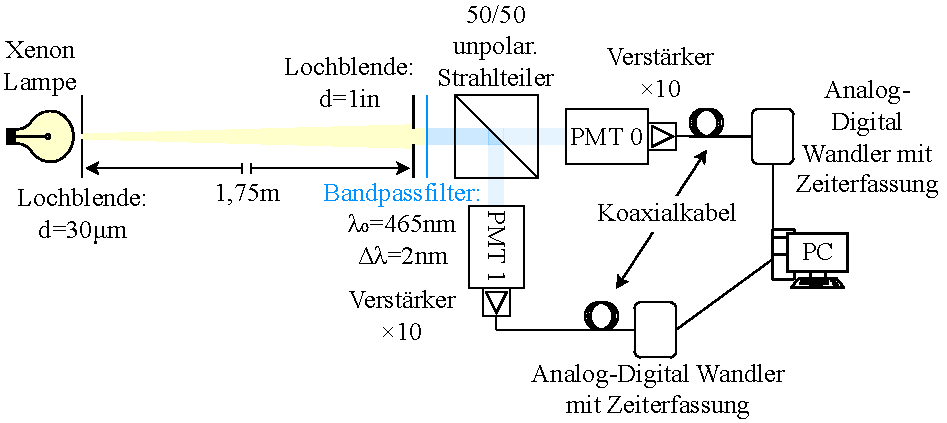
\includegraphics[width=0.9\linewidth]{images/Aufbau/Aufbau.pdf}
    \caption{Gezeigt ist eine vereinfachte Skizze des verwendeten Aufbaus, welche die konzeptuell wichtigsten Bestandteile darstellt.}
    \label{fig:Versuchsaufbau}
\end{figure}
Als Lichtquelle wird eine Xenonlampe (Osram XBO 75 W/2 \cite{XBO75OSRAM}) gewählt. 
Als Gasentladungslampe emittiert diese nach \autoref{ssec:Intensitätsinterferometrie} chaotisches Licht, welches Bunching aufweist. 
Da nach dem van Cittert-Zernike-Theorem der Winkeldurchmesser der Lichtquelle invers proportional zur Breite von $g^{(2)}(\bm{\rho})$ ist, ist weiterhin darauf zu achten, die Ausdehnung der Lichtquelle einzuschränken, damit korrelierte Photonen am Detektor vorliegen. 
Zu diesem Zweck ist eine kreisförmige Lochblende mit einem Durchmesser von $d=30\,\mathrm{\mu m}$ verbaut. 
Mit der Distanz $x=1{,}75\,\mathrm{m}$ zwischen Lichtquelle und dem restlichen Aufbau ergibt sich so ein Winkeldurchmesser von $\Delta \theta \approx \frac{d}{x} = 3{,}53\,\mathrm{arcsec}$. 
Es sei darauf hingewiesen, dass typische Winkeldurchmesser von Sternen im Bereich von tausendstel Bogensekunden liegen \cite{hanburybrownAngularDiameters321974}, also etwa drei Größenordnungen kleiner sind, als der hier geschaffene \glqq künstliche Stern\grqq. \\
Um dem eintretenden Lichtstrahl eine definierte Breite zu geben, wird dieser zusätzlich durch eine Lochblende mit einem Durchmesser von einem Zoll geleitet. 
Weiterhin wird das einfallende Licht so auf einen Bereich beschränkt, der etwa der effektiven Größe der Photomultiplier von $23\times 23\,\mathrm{mm}$ entspricht \cite{PhotomultiplierTubeR11265U200}. \\
Wie in \autoref{ssec:Michelson-Sterninterferometer} beschrieben, ist für eine Messung der räumlichen Kohärenz auch eine nicht verschwindende Kohärenzzeit relevant. 
Da diese indirekt proportional zur spektralen Breite der Quelle ist, wird an dieser Stelle ein enger Bandpassfilter (Alluxa 465-2 \cite{4652OD4Ultra}) mit einer annähernd rechteckförmigen Transmissivität verbaut. 
Dieser hat nach Herstellerangaben eine zentrale Wellenlänge von $\lambda_0 = 465\,\mathrm{nm}$ und eine Halbwertsbreite von  $\Delta\lambda = 2\,\mathrm{nm}$. 
Anschließend wird der Strahl durch einen nicht polarisierenden 50/50 Strahlteilerwürfel (Thorlabs BS031 \cite{ThorlabsBS03150}) aufgeteilt und zum Nachweis der Photonen auf zwei Photomultiplier (PMTs, Hamamatsu R11265U-200 \cite{PhotomultiplierTubeR11265U200}) gelenkt. 
Um bei hohen Photonenraten weiterhin eine lineare Verstärkung durch die PMTs zu erhalten, werden die letzten vier Dynoden mit einer Stabilisationsspannung betrieben \cite{zmijaOpticalIntensityInterferometry2021}. 
Als Spannungsquelle für die Hochspannung und die Stabilisationsspannung wird eine durch den Computer steuerbare Spannungsquelle (CAEN DT5533E \cite{DT5533E}) genutzt. 
Direkt am Ausgang der Photomultiplier werden die Pulse mit einem Verstärker (FAST ComTec TA1000B-10 \cite{TA1000BTimingAmplifier}) um den Faktor 10 verstärkt. 
Die Verstärkung direkt an den PMTs hat den Vorteil, dass Störsignale nicht vor der Verstärkung einkoppeln können, was das Signal-Rausch-Verhältnis verbessert. 
Anschließend werden die Signale durch variable Kombinationen an Kabellänge und -modell zu Analog-Digital-Wandlern (Spectrum M4I.2212-X8 \cite{M4i2212x8Bit} und Spectrum M4I.2211-X8 \cite{M4i2211x8Bit}, gleiches Modell, lediglich unterschiedlich viele Eingangskanäle) geleitet, wo diese digitalisiert werden. 
Obwohl die Spektrum-Karten vier bzw. zwei Digitalisierungskanäle unterstützen, werden zwei verschiedene und räumlich getrennte Karten genutzt, um ein Übersprechen zwischen den Kanälen zu verhindern. 
Aufgrund des von Natur aus geringen Signals werden alle analogen Signale durch geschirmte Koaxialkabel geleitet, um das Einkoppeln von Störsignalen zu erschweren. 
Um zusätzlich das Einkoppeln von störendem Licht des PCs oder sonstiger LEDs der Messgeräte zu erschweren, ist der optische Aufbau zudem durch ein Thorlabs-Röhrensystem fest verbunden, sodass nur Licht entlang der optischen Achse eindringen kann. 
Die zeitliche Synchronisierung der beiden des PMT-Strom-Verläufe (Waveforms) zur späteren Korrelation erfolgt durch Verwendung des White Rabbit Systems (vgl. z. B. \cite{lipinskiWhiteRabbitPTP2011}), welches direkt mit den Analog-Digital-Wandlern (ADCs) verbunden ist. 
Abschließend werden die Daten auf RAIDs (Areca ARC-8050T3U-12 \cite{ARC8050T3UThunderboltUSB}) zur späteren Korrelation gespeichert. \\
Da ein Ziel dieser Arbeit ist, zu untersuchen, wie sich verschiedene Kabel auf das Integral des Bunching Peaks auswirken, soll an dieser Stelle explizit auf die verwendeten Koaxialkabel eingegangen werden. 
Die ersten durchgeführten Messungen erfolgen mit 10 und 40\,m langen Kabeln des Typs Airborne 5 \cite{s.r.lAirborne10Coaxial}. 
Dies entspricht den Kabeln, welche in der von der Arbeitsgruppe 2022 durchgeführten Kampagne mit den H.E.S.S.-Teleskopen genutzt wurden \cite{zmijaFirstIntensityInterferometry2023}. 
Anschließend wurden noch Messungen mit Kabeln des Typs LMR 400 durchgeführt \cite{LMR400CoaxCable}. 
Diese weisen eine geringere Dämpfung auf als die Airborne 5 Kabel und sind daher interessant, um den Einfluss der Dämpfung auf das gemessene $\tau_{\mathrm{c}}$ zu untersuchen. \\

Aufgrund des speziellen Aufbaus ergeben sich einige Änderungen bezüglich der im vorangegangenen Abschnitt eingeführten Theorie. 
Auf diese soll hier eingegangen werden. 
Wie erwähnt ist der Winkeldurchmesser der Quelle vergleichsweise groß. 
Nach \autoref{eq:erste nulstelle von g2(rho) für lochblende} wird für die Distanz zur ersten Nullstelle der $g^{(2)}$-Funktion lediglich $\rho_0\approx3{,}3\,\mathrm{cm}$ erwartet. 
Das heißt, dass am Beobachtungsort lediglich zwischen Punkten, die maximal $\rho_0$ voneinander entfernt sind, korrelierte Photonen auftreten. 
Aufgrund der physischen Größe der PMTs ist es daher nicht möglich, $g^{(2)}(\rho)$ für verschiedene $\rho$ zu messen. 
Stattdessen wird ein Mittelwert von $g^{(2)}$ in einem Intervall von $\rho\in[0,1]$ Zoll gemessen. 
Dieses Intervall entspricht den Abständen, die korrelierte Photonen durch die Lochblende am Eingang des Strahlteilers haben können. 
Es wird also erwartet, einen niedrigeren Wert für $g^{(2)}(\rho)$ und damit $\tau_{\mathrm{c}}$ zu messen. 
Dies ist in \autoref{fig:räumliche koh simulation} verdeutlicht. 
Um herauszufinden, um welchen Faktor die gemessene Amplitude von der theoretischen maximalen Amplitude abweicht, wird eine von der Arbeitsgruppe geschriebene Simulation durchgeführt, die sowohl den Wert von $g^{(2)}$ für jeden Photonenabstand als auch die Wahrscheinlichkeit für diesen berücksichtigt. 
Der Faktor, um welchen $g^{(2)}$ im Vergleich zu $g^{(2)}(0)$ verringert ist, beträgt bei gegebenem Aufbau $k_\mathrm{T}=0{,}62$. 
Über den theoretischen Verlauf der Korrelationsfunktion lässt sich durch $k_\mathrm{T}$ auf einen effektiven Teleskopabstand $\rho\prime$ schließen, bei dem ein dünner Strahl denselben Verlust an räumlicher Kohärenz aufweist. 
Dies ist auch in \autoref{fig:räumliche koh simulation} veranschaulicht. 
\begin{figure}[ht]
    \centering
    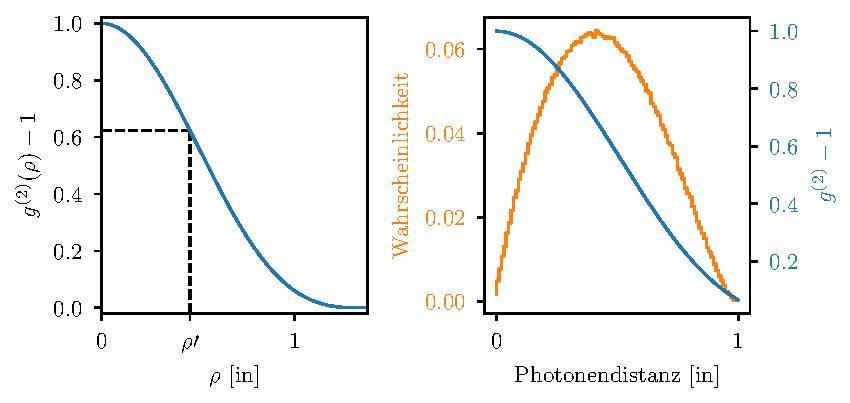
\includegraphics{images/Aufbau/g2(rho).pdf}
    \caption{Dargestellt ist links die $g^{(2)}$-Funktion, abhängig von der Separation $\rho$. Rechts ist das Ergebnis der Simulation abgebildet. In Blau ist $g^{(2)}$ für jeden Photonenabstand dargestellt (dies entspricht der Kurve im linken Graphen), während in Orange die simulierte Wahrscheinlichkeitsverteilung, ein Photonenpaar bei gegebenem Abstand anzutreffen, aufgetragen ist. Durch Multiplikation der beiden Kurven erhält man den Faktor, wie viel räumliche Kohärenz im Vergleich zum Maximum noch vorhanden ist. Dieser beträgt $k_\mathrm{T}=0{,}62$. Links ist zudem eingezeichnet, welchem Abstand $\rho\prime$ diese Kohärenz entsprechen würde. }
    \label{fig:räumliche koh simulation}
\end{figure}

Aus voriger Überlegung ist nun bekannt $\tau_{\mathrm{c}}^{\mathrm{expect}} = k_\mathrm{T}\cdot\tau_{\mathrm{c}}^{\mathrm{th}}$. 
Um den Theoriewert bei perfekter räumlicher Kohärenz $\tau_{\mathrm{c}}^{\mathrm{th}}$ zu bestimmen, wird eine weitere Simulation von der Arbeitsgruppe verwendet. 
Diese berechnet aus dem vom Hersteller gegebenen Transmissionspektrum des Filters über das Wiener-Khintchine-Theorem, d. h. eine Fouriertransformation, die erwartete $g^{(1)}$-Funktion, welche anschließend über die Siegert-Relation in $g^{(2)}(\tau, \rho=0)$ umgerechnet wird. 
Daraus folgt dann für den vorliegenden Fall $\tau_{\mathrm{c}}^{\mathrm{th}} = \int \left(g^{(2)}(\tau, \rho=0) -1\right) d\tau = 0{,}152\,\mathrm{ps}$. 
Abschließend ergibt sich also für die erwartete Kohärenzzeit bei verwendetem Aufbau:
\begin{equation}
    \tau_{\mathrm{c}}^{\mathrm{expect}} = 0{,}62 \cdot 0{,}152\,\mathrm{ps} = 94\,\mathrm{fs}
    \label{eq:tau_c_th}
\end{equation}

Da in den Faktor $k_\mathrm{T}$ der Winkeldurchmesser der Quelle und damit auch der Durchmesser der Lochblende nach der Xenonlampe eingeht und diese starker Hitze ausgesetzt ist, wurde zudem überprüft, ob die Herstellerangaben von 30\,$\mathrm{\mu m}$ noch zutreffen. 
Eine Aufnahme der Lochblende unter dem Mikroskop ist dafür in \autoref{fig:lochblende mikroskop} gezeigt. 
\begin{figure}[h]
    \centering
    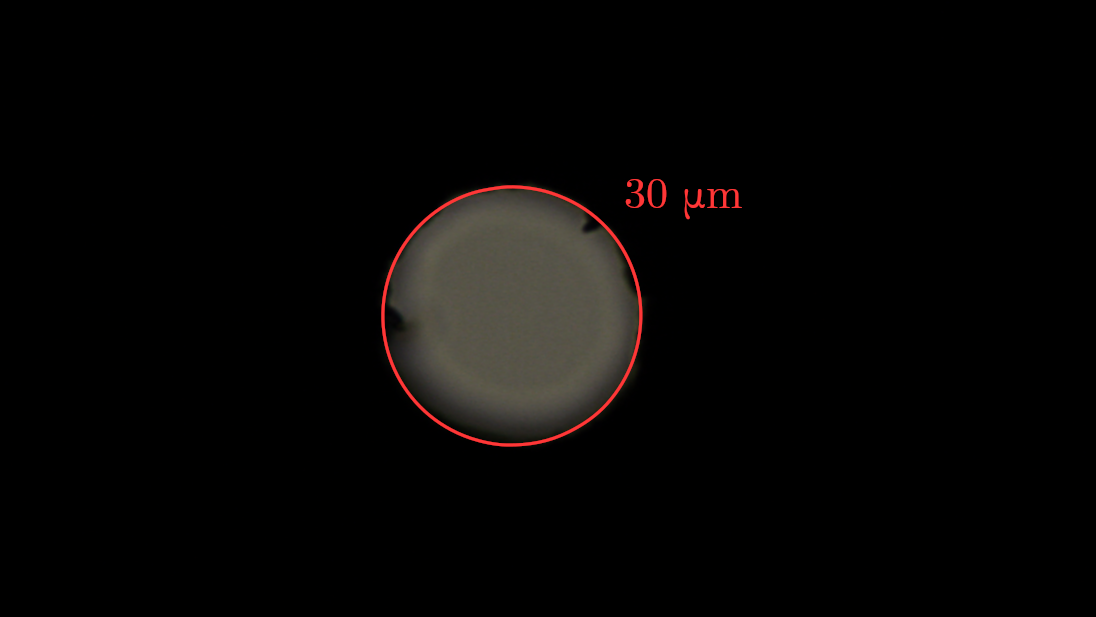
\includegraphics[width=0.8\textwidth]{images/Aufbau/Lochblende_Mikroskop.png}
    \caption{Die Mikroskopaufnahme der Lochblende sowie ein Kreis mit $30\,\mathrm{\mu m}$-Durchmesser sind gezeigt. Trotz irregulärer Strukturen am Rand entspricht der gemessene Durchmesser recht genau den Herstellerangaben.}
    \label{fig:lochblende mikroskop}
\end{figure}
Der eingezeichnete Kreis entspricht einem Durchmesser von $30\,\mathrm{\mu m}$. 
Auch wenn deutliche Abnutzungserscheinungen an den Rändern sichtbar sind, ist der gemessene Durchmesser sehr nah an den $30\,\mathrm{\mu m}$, die in die Berechnung von $k_\mathrm{T}$ eingehen. 
Der erwähnte Wert von $\tau_{\mathrm{c}}^{\mathrm{expect}}$ entspricht daher der Erwartung an die Messung und muss nicht noch zusätzlich wegen eines abweichenden Lochblendendurchmessers angepasst werden. 

\clearpage

\section{Datenaufnahme und Pre-Processing}
\label{sec:Datenaufnahme und Pre-Processing}
In diesem Abschnitt soll auf die Datenaufnahme sowie alle nötigen Schritte der Datenverarbeitung bis zur fertigen $g^{(2)}(\tau)$-Funktion eingegangen werden. 
Dafür werden zuerst die Datenaufnahme und dafür nötige Kalibrationsverfahren erläutert. 
In diesem Zuge wird zudem auf das Aussehen der aufgenommenen Daten (Waveforms) eingegangen. 
Anschließend werden korrelierte Einzeldateien betrachtet und es wird verdeutlicht, warum eine Mittelung vieler Waveforms unumgäglich ist. 
Zuletzt werden angewandte Korrekturen und Filter angesprochen sowie verdeutlicht, wie die Mittelung der Daten erfolgt. 

\subsection{Datenaufnahme und Waveforms}
\label{ssec:Datenaufnahme und Waveforms}
Die Aufnahme der Daten erfolgt durch ein von der Arbeitsgruppe geschriebenes Programm, welches mit den ADCs kommuniziert. Ein Screenshot der GUI, auf dem die wichtigsten Schritte der Datenaufnahme markiert sind, ist in \autoref{fig:Screenshot GUI} eingefügt. 
\begin{figure}[h]
    \centering
    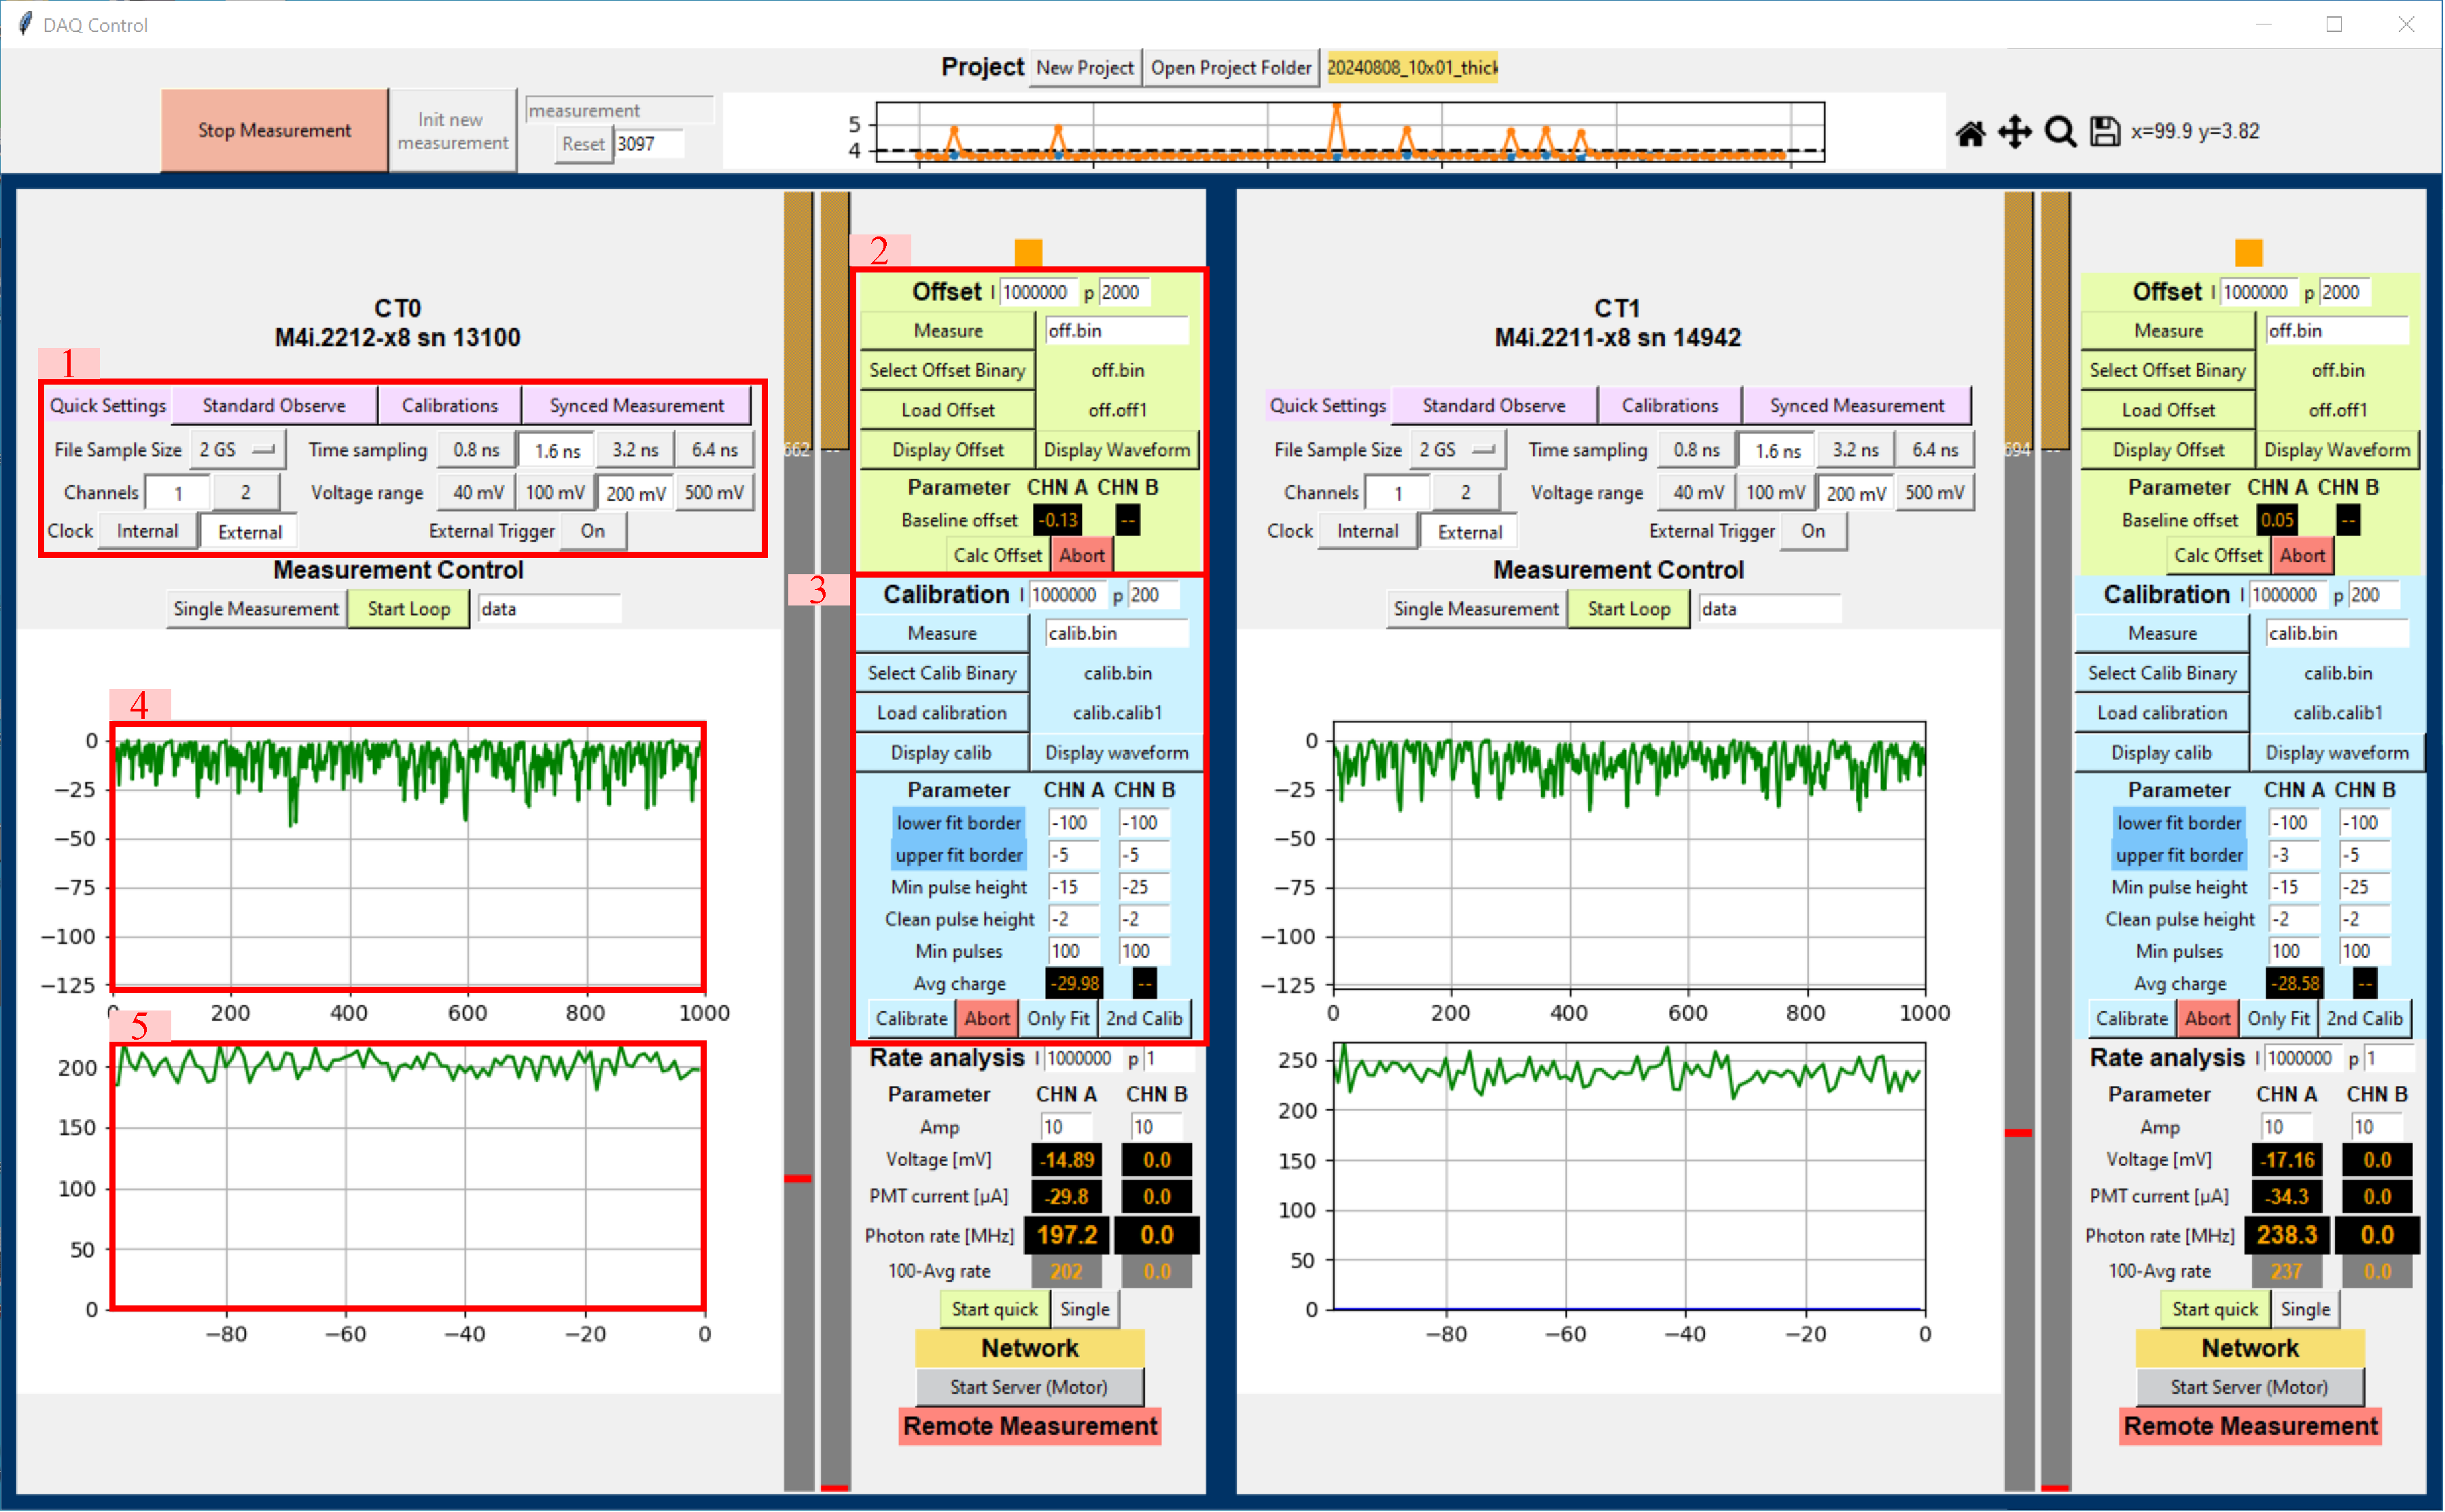
\includegraphics[width=0.9\textwidth]{images/Datenaufnahme/GUI.pdf}
    \caption{Dargestellt ist ein Screenshot der GUI zur Datenaufnahme. Wichtige Schritte sind markiert.}
    \label{fig:Screenshot GUI}
\end{figure}
In der GUI wird für jede verwendete Digitalisierungskarte ein Fenster erstellt, in dem Einstellungen für die jeweilige Karte vorgenommen werden können. 
Nach dem Erstellen eines Projekts können in dem mit \emph{1} markierten Bereich in \autoref{fig:Screenshot GUI} Einstellungen für die ADC-Karte vorgenommen werden. 
Es wird mit einem Kanal je Karte gemessen und die Samplingzeit beträgt $1{,}6$\,ns bei einer Dateigröße von 2 Gigasamplen. 
Der zu digitalisierende Spannungsbereich wird passend zu den in \emph{4} abgebildeten Waveforms auf 200\,mV gesetzt. 
Clock und Trigger werden extern durch das White Rabbit System gegeben. 
Die genannten Einstellung werden größtenteils vor der Messung automatisch mit dem Button \glqq Init new measurement\grqq\;gesetzt. \\
Vor Start der Messung müssen zwei Kalibrationsschritte für jeden Kanal gemacht werden. 
Zuerst wird unter \emph{2} eine Offset-Kalibration durchgeführt, indem \glqq Measure\grqq\;und \glqq Calc Offset\grqq\;gewählt werden. 
Diese wird ohne Beleuchtung und mit ausgeschalteter Hochspannung durchgeführt. 
Das Programm bestimmt diesen vom PMT abhängigen Offset und entfernt diesen, sodass dieser die Korrelation nicht beeinflusst \cite{zmijaOpticalIntensityInterferometry2021}. 
Anschließend wird bei eingeschalteter Hochspannung und niedriger Photonenrate eine Raten-Kalibration durchgeführt, sodass gemessene Spannungen in Photonenraten umgerechnet werden können. 
Dies ist nötig, da aufgrund der hohen Raten bei der Messung nicht Einzelphotonepulse, sondern ganze Waveforms miteinander korreliert werden. 
Für die Kalibration wird für jeden Kanal die mittlere Pulsform der PMT-Pulse bestimmt und gespeichert. 
Es wird erwartet, dass diese einen bedeutenden Einfluss auf die Form der $g^{(2)}$-Funktion hat, da die Photonenpulse deutlich breiter sind als die einzelnen $1{,}6$\,ns-Bins, was zu einer Korrelation benachbarter Bins führt \cite{zmijaOpticalIntensityInterferometry2021}. 
Aus den gemessenen Daten wird bestimmt, wie viel Ladung ein Photon, das auf einen PMT trifft, durchschnittlich freisetzt, woraus anschließend die in \emph{5} gezeigten Photonenraten in MHz bestimmt werden können. \\
Nach diesen Kalibrationsschritten kann die Messung gestartet werden, woraufhin synchronisiert durch den Trigger des White Rabbit Systems 2$\cross$2\,GS Daten aufgenommen werden. 
Dies entspricht einer Messdauer von $3{,}436\,\mathrm{s}$. 
Nach Ablauf von 4\,s startet anschließend der nächste Trigger eine Messung von 2$\cross$2\,GS, sodass idealerweise ein Duty-Cycle von 85{,}9\% erreicht wird \cite{zmijaFirstIntensityInterferometry2023}. 
Da jedes Sample einem 8\,bit ADC-Wert entspricht, erreicht die Messung also eine Datenrate von 2$\cross$2\,GB alle 4\,s, was erklärt, weshalb die Daten erst gespeichert und anschließend offline korreliert werden. 
Zur Veranschaulichung ist in \autoref{fig:Offest_Rate Kalibration} aufgezeigt, wie eine typische Waveform zur Offset- bzw. Raten-Kalibration und zur Messung aussieht. 
\begin{figure}[h]
    \centering
    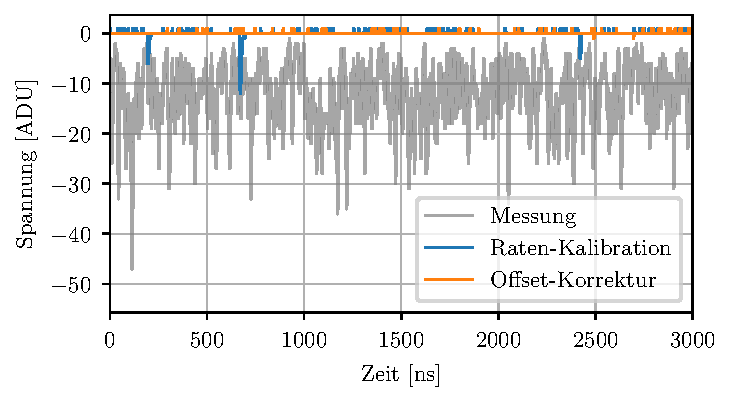
\includegraphics{images/Datenaufnahme/Kalibration.pdf}
    \caption{Abgebildet ist der Ausschnitt einer Waveform für die Offset Kalibration (ausgeschaltete Hochspannung und Beleuchtung), Raten-Kalibration (Hochspannung und Licht an, niedrige Photonenrate) und für die Messung.}
    \label{fig:Offest_Rate Kalibration}
\end{figure}

\subsection{Korrelation}
\label{ssec:Korrelation}
Die Korrelation der Daten erfolgt parallelisiert, nachdem die Datenaufnahme abgeschlossen ist. 
Jede Datei von beiden Kanälen wird getrennt miteinander korreliert, indem diese zuerst in Vektoren $\mathbf{A}$ und $\mathbf{B}$ eingelesen werden. 
Anschließend wird für jede Zeitdifferenz $\tau$ das folgende Skalarprodukt berechnet: 
\begin{equation}
    G^{(2)}(\tau) = \mathbf{A}(t)\cdot\mathbf{B}(t+\tau)
    \label{eq:korrelation}
\end{equation}
Damit entspricht jeder Wert von $G^{(2)}(\tau)$ der unnormierten zeitlichen Photonenkorrelation zu diesem Zeitpunkt \cite{zmijaOpticalIntensityInterferometry2021}. 
Die korrelierten Einzeldateien können anschließend für die weitere Datenanalyse gespeichert werden, da diese deutlich kleiner (im Bereich weniger kB) sind als die Rohdaten. 
Um aus einer bestimmten $G^{(2)}$-Funktion die normierte zeitliche Korrelationsfunktion zu erhalten, wird diese durch ihren Mittelwert weit außerhalb des Bunching Peaks geteilt:
\begin{equation}
    g^{(2)}(\tau) = \frac{G^{(2)}(\tau)}{\overline{G^{(2)}(\tau\gg\tau_c)}}
    \label{eq:G2 normalisierung}
\end{equation}
Ein Beispiel für die unnormierte Funktion $G^{(2)}$ einer einzelnen Datei ist in \autoref{fig:G2(tau)} dargestellt. 
\begin{figure}[h]
    \centering
    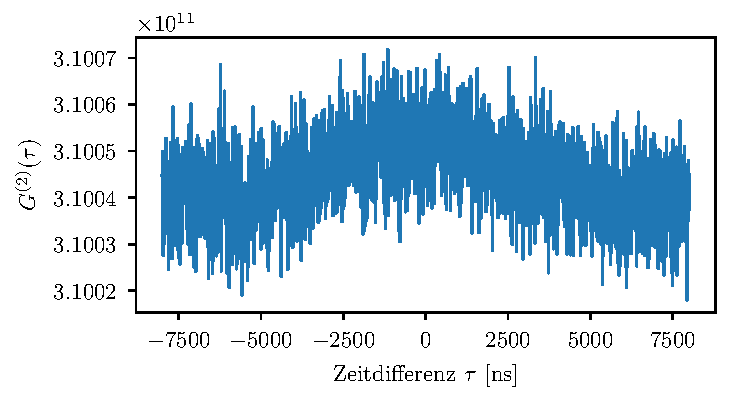
\includegraphics{images/Datenaufnahme/G2.pdf}
    \caption{Ein Beispiel einer unnormierten Korrelationsfunktion ist abgebildet. Durch das verrauschte Signal ist an der Stelle $\tau=0$ kein Bunching Peak sichtbar.}
    \label{fig:G2(tau)}
\end{figure}
Es ist ersichtlich, dass die Funktion stark verrauscht ist und der Bunching Peak nicht auszumachen ist. 
Die in \autoref{ssec:Intensitäteninterferometrie} bereits erwähnte Nowendigkeit der Mittelung über viele Daten, d. h. lange Zeiten, um die Form von $g^{(2)}$ bestimmen zu können, ist daher deutlich sichtbar. 

\subsection{Mittelung der Daten und Filter}
\label{ssec:mittelung und filter}
Wie bereits im vorangegangenen Abschnitt ersichtlich wurde, ist eine Mittelung vieler Dateien unumgänglich, um den Bunching Peak analysieren zu können. 
Hierbei wird der Ansatz eines gewichteten Mittelwerts gewählt, da nicht jede der etwa $3{,}4\,\mathrm{s}$ langen Dateien statistisch gleich aussagekräftig ist. 
So weisen manche der Messabschnitte höhere Photonenraten auf als andere (vgl. dazu \autoref{fig:Screenshot GUI}, Kasten \emph{5}). 
Unter der Annahme, dass ein Großteil des Rauschens in der $G^{(2)}$-Funktion statistischen Fluktuationen entspricht, wird erwartet, dass das Rauschen für höhere Photonenraten abnimmt. 
Dies bedeutet, dass Dateien mit höheren Raten und geringerer Schwankung stärker gewichtet werden sollten, als jede mit geringeren Photonenraten. 
Um dies zu bewerkstelligen, wird von jeder Datei $G^{(2)}_i$ die Standardabweichung $\sigma_i$ bestimmt und anschließend der folgende gewichtete Mittelwert berechnet \cite{cochranProblemsArisingAnalysis1937}:
\begin{equation}
    \overline{G^{(2)}} = \frac{\sum_{i=0}^{n}\frac{G^{(2)}_i}{\sigma_i^2}}{\sum_{i=0}^{n} \sigma_i^{-2}}
\end{equation}
Das Ergebnis der Mittelung über 10000 Dateien, d. h. etwa $9{,}5$\,h Korrelationsdaten, ist in \autoref{fig:gemittelte G2 vs g2} oben abgebildet. 
Der Bunching Peak bei $\tau\approx 0$ ist nach Mittelung der Daten bereits sichtbar. 
Allerdings sind durch die Mittelung weitere Artefakte ersichtlich geworden. 
Bereits in den korrelierten Einzeldateien ist eine Struktur in den Daten zu erkennen, welche das Signal überlagert. 
Nach der Mittelung ist diese nun besonders deutlich, was darauf hinweist, dass sie nicht von rein statistischer Natur ist, sondern tatsächlich zwischen den Kanälen korreliert ist. 
Das etwa $12\,\mathrm{\mu s}$ breite Störsignal kommt von der Spannungsversorgung der Xenonlampe \cite{zmijaOpticalIntensityInterferometry2021}, liegt daher in beiden Kanälen zugleich vor und wird deshalb durch die Korrelation und Mittelung verstärkt. 
Da es aber mehrere Größenordnungen breiter ist als der Bunching Peak und diesen daher kaum beeinflusst, wird es in diesem Abschnitt erst einmal vernachlässigt. 
In einem späteren Abschnitt zur Integration des Peaks wird auf eine Methode eingegangen, dieses Störsignal zu entfernen. \\
\begin{figure}[h]
    \centering
    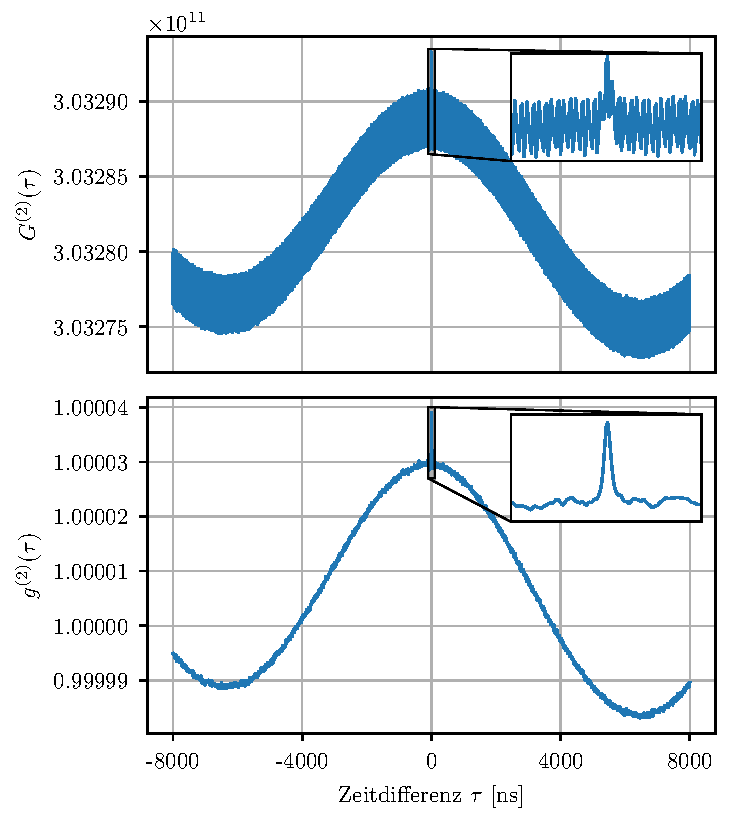
\includegraphics{images/Datenaufnahme/G2_vs_g2.pdf}
    \caption{Dargestellt sind der Unterschied zwischen $G^{(2)}(\tau)$ und der normierten Funktion $g^{(2)}(\tau)$ nach Mittelung über 10000 Dateien, bei der zudem die \glqq pattern correction\grqq\;und der Tiefpass angewandt worden sind. Es ist deutlich erkennbar, dass die angewandten Methoden zu einer starken Verbesserung des Signal-Rausch-Verhältnisses geführt haben. }
    \label{fig:gemittelte G2 vs g2}
\end{figure}

Weiterhin ist durch Zoom in die Daten oder eine Fouriertransformation dieser ein 8-Bin-periodisches Muster zu erkennen, welches dafür verantwortlich ist, dass die $G^{(2)}$-Funktion ein breites Band an Werten annimmt. 
Dieses von den ADC-Karten kommende Muster stört den Verlauf des Bunching Peaks zudem in beträchtlicher Weise, da es sich auf der selben Zeitskala wie der Peak selbst befindet. 
Da das Störsignal von den beiden ADC-Karten gleichzeitig ausgeht, ist dieses korreliert und daher besonders dominant in der abgebildeten $G^{(2)}$-Funktion.
Um das Störsignal zu entfernen, wird eine von der Arbeitsgruppe geschriebene \glqq pattern correction\grqq\;angewandt, welche in den ersten 4000 Bins (d. h. im Intervall $\tau\in[-8000,-1600]\,\mathrm{ns}$) jeweils 8 Bins mittelt und die Daten anschließend durch das so ermittelte Muster teilt. 
Da das Muster sowohl das eigentliche 8-Bin-periodische Muster, als auch den Offset der $G^{(2)}$-Funktion, wie er in \autoref{eq:G2 normalisierung} definiert ist, enthält, wird diese durch die Division automatisch auch normiert. 
Der Schritt der \glqq pattern correction\grqq\;wird für jede Datei separat vor der Bildung des Mittelwertes angewandt. \\
Nach diesen Schritten wird auf die gemittelte $g^{(2)}$-Funktion noch ein digitaler Tiefpass 2. Ordnung mit einer Grenzfrequenz von 200\,MHz angewandt, um weitere hochfrequente Störsignale zu entfernen. 
Die nach erwähnten Korrekturen und der angewandten Mittelung erhaltene Funktion $g^{(2)}(\tau)$ ist in \autoref{fig:gemittelte G2 vs g2} unten abgebildet. 


\clearpage
%---------------------------------------------------------
%	Acronyms
%---------------------------------------------------------

% \clearpage
% \mbox{}
% \clearpage
% \printnoidxglossary[type=acronym]
% \printacronyms
% \clearpage

%---------------------------------------------------------
%	Appendix (if needed)
%---------------------------------------------------------
% \clearpage
% \mbox{}
% \clearpage
% \appendix
% \addtocontents{toc}{\protect\setcounter{tocdepth}{1}}
% \addtocontents{toc}{\protect\renewcommand{\protect\sectionautorefname}{Appendix}}
% \newgeometry{
% 	%a4paper,
% 	left=40mm,
%     % right=20mm,
% 	top=15mm,
% }
%     
\section{Appendix A}
Your appendix goes here!



%---------------------------------------------------------
%	Bibliography
%---------------------------------------------------------

\clearpage
\mbox{}
\clearpage

\newgeometry{
	%a4paper,
	left=40mm,
    % right=20mm,
	top=35mm,
}
\renewcommand\refname{Bibliography}
% \printbibliography
\printbibliography[
heading=bibintoc,
title={Bibliografie}
]

%---------------------------------------------------------
%	Danksagung
%---------------------------------------------------------

% \clearpage
% \mbox{}
% \clearpage

% \section*{Danksagung}
Here you can thank everyone you want to. 
% 
\begin{itemize}
    \item Max Mustermann for having a name that is simple to remember.
    \item Dr. Albert Einstein for having fun ideas about space-time.
\end{itemize}


% \clearpage
%---------------------------------------------------------
%	Eigenständigkeitserklärung / Declaration of independence
%---------------------------------------------------------

% \selectlanguage{german}
% \section*{Eigenständigkeitserklärung}
% Hiermit versichere ich, Stephen Weybrecht (22967286), die vorgelegte Arbeit selbstständig und ohne unzulässige Hilfe Dritter sowie ohne die Hinzuziehung nicht offengelegter und insbesondere nicht zugelassener Hilfsmittel angefertigt zu haben. Die Arbeit hat in gleicher oder ähnlicher Form noch keiner anderen Prüfungsbehörde vorgelegen und wurde auch von keiner anderen Prüfungsbehörde bereits als Teil einer Prüfung angenommen.\\

% Die Stellen der Arbeit, die anderen Quellen im Wortlaut oder dem Sinn nach entnommen wurden, sind durch Angaben der Herkunft kenntlich gemacht. Dies gilt auch für Zeichnungen, Skizzen, bildliche Darstellungen sowie für Quellen aus dem Internet.\\

% Mir ist insbesondere bewusst, dass die Nutzung künstlicher Intelligenz verboten ist, sofern diese nicht ausdrücklich als Hilfsmittel von dem Prüfungsleiter bzw. der Prüfungsleiterin zugelassen wurde. Dies gilt insbesondere für Chatbots (insbesondere ChatGPT) bzw. allgemein solche Programme, die anstelle meiner Person die Aufgabenstellung der Prüfung bzw. Teile derselben bearbeiten könnten.\\

% \vspace{10cm}
% \begin{flushleft}
% \makebox[.4\textwidth]{\hrulefill}\hfill \makebox[.4\textwidth]{\hrulefill}\\
% \makebox[.4\textwidth]{Ort, Datum}\hfill
% \makebox[.4\textwidth]{Unterschrift}\\
% \end{flushleft}


\end{document}

